%%-----------------------------------------------------------------------
% Loading the packages and classes
%%-----------------------------------------------------------------------

\documentclass[12pt,twoside,a4paper,final]{book}%
\usepackage{a4}%                        %% Verwendet mehr Platz auf einer A4 Seite als Option a4paper in book
\usepackage[english,ngerman]{babel}%    %% Babel Sprachen
\usepackage[latin1]{inputenc}%          %% input encoder f�r umlaute usw.
\usepackage[T1]{fontenc}
\usepackage{amssymb}%                   %% AMS Symbole
\usepackage{amsmath}%                   %% AMS Math Funktionen
\usepackage{amsfonts}%
\usepackage[Sonny]{fncychap}%           %% Chapter Style
\usepackage[english,noprefix]{nomencl}%  %% Nomenclature (Symbolverzeichnis)
\usepackage{makeidx}%                   %% Index
\usepackage{graphicx}%                  %% Graphiken
\graphicspath{{img/}}
\DeclareGraphicsExtensions{.pdf,.jpeg,.png,.jpg}
\usepackage{psfrag}%                    %% Tex-Schriftarten und Formeln in EPS-Grafiken
\usepackage{color}
\usepackage{nicefrac}
\usepackage{ifthen}
\usepackage{fancyhdr}
\usepackage{subfigure}
\usepackage[xindy, acronym, toc]{glossaries}
\usepackage{cite}
\usepackage{listings}
\usepackage{color}
\usepackage[dvipsnames]{xcolor}
\usepackage{rotating}
\usepackage{multirow}
\usepackage{eurosym}
\usepackage{capt-of}


%Define Acronyms like
% use on every place in your document \gls{mas} for TGM or - for plural - use \glspl for TGMs
% at the first usage of this, the acronym will be introduced, everywhere else it will only be the in the short form: ``Technologisches Gewerbemuseum (TGM)''
% TIPP: USE THIS FOR EVERY NAME/SOFTWARE-TOOL/MAIN PART OF YOUR WORK, like JAVA, - so that, e.g. JAVA is not written Java everywhere else in your thesis.

\newacronym{tgm}{TGM}{Technologisches Gewerbemuseum}
\newacronym{fp}{FP-Analyse}{Function-Point-Analyse}
\newacronym{pm}{PM}{Personenmonate}

\newacronym{ma}{MA}{Moving Average}
\newacronym{sma}{SMA}{Simple Moving Average}
\newacronym{lwma}{LWMA}{Linear Weighted Moving Average}
\newacronym{wma}{WMA}{Linear Weighted Moving Average}
\newacronym{ema}{EMA}{Exponential Moving Average}
\newacronym{ama}{AMA}{Adaptive Moving Average}
\newacronym{tma}{TMA}{Triangular Moving Average}
\newacronym{er}{ER}{Efficiency Ratio}
\newacronym{dema}{DEMA}{Double Exponential Moving Average}
\newacronym{tema}{TEMA}{Triple Exponential Moving Average}
\newacronym{adx}{ADX}{Average Directional Movement Index}
\newacronym{sf}{SF}{Smoothing Factor}
\newacronym{macd}{MACD}{Moving Average Convergence/Divergence}
\newacronym{cci}{CCI}{Commodity Channel Index}
\newacronym{rsi}{RSI}{Relative Strength Indicator}

\newacronym{forex}{FOREX}{Foreign Exchange Market}
\newacronym{hft}{HFT}{High Frequency Trading}

\newacronym{bts}{BTS}{Backtesting-Software}
\newacronym{git}{GIT}{GIT-Server}
\newacronym{ide}{IDE}{Integrated Development Environment}
\newacronym{mql5}{MQL5}{MetaQuotes Language 5}
\newacronym{gui}{GUI}{Graphical User Interface}
\newacronym{dll}{DLL}{Dynamic Link Library}
\newacronym{xml}{XML}{eXtensible Markup Language}
\newacronym{xaml}{XAML}{eXtensible Application Markup Language}
\newacronym{clr}{CLR}{Common Language Runtime}
\newacronym{cls}{CLS}{Common Language Specification}
\newacronym{wpf}{WPF}{Windows Presentation Foundation}
\newacronym{jvm}{JVM}{Java Virtual Machine}
\newacronym{api}{API}{Application Programming Interface}
\newacronym{mvvm}{MVVM}{Model View Viewmodel}
\newacronym{soap}{SOAP}{Simple Object Access Protocol}
\newacronym{linq}{LINQ}{Language Integrated Query}
\newacronym{sql}{SQL}{Structured Query Language}
\newacronym{csv}{CSV}{Comma-separated values}

\newacronym{afa}{AFA}{Abschreibung f�r Abnutzung}
%%-----------------------------------------------------------------------
% Using the Hyperref-Package for PDF-Online Version
%%-----------------------------------------------------------------------

\def\usehyperref{1}

\ifnum\usehyperref=1
\usepackage[pdftex=true,
  pdftitle={Diplomarbeit},
  pdfauthor={Gottfried Koppensteiner},
  bookmarksopen,
  colorlinks,
  citecolor=blue,
  linkcolor=blue,
  breaklinks%
]{hyperref}%
\fi



%%-----------------------------------------------------------------------
% Rearranging Nomenclature
%%-----------------------------------------------------------------------


\renewcommand{\nomname}{List of symbols}
%\renewcommand{\nompreamble}{The following list only contains symbols
%  that are used continuously throughout the text. Local symbols are
%  not listed.}
\renewcommand{\nomgroup}[1]{
 \ifthenelse{\equal{#1}{A}}{\item[\textbf{General symbols}\bigskip]}{
 \ifthenelse{\equal{#1}{B}}{\item[\bigskip\bigskip\textbf{Chapter 2}\bigskip]}{
 \ifthenelse{\equal{#1}{C}}{\item[\bigskip\bigskip\textbf{Chapter 3}\bigskip]}{
 \ifthenelse{\equal{#1}{D}}{\item[\bigskip\bigskip\textbf{Chapter 4}\bigskip]}{
 \ifthenelse{\equal{#1}{E}}{\item[\bigskip\bigskip\textbf{Chapter 5}\bigskip]}{
 \ifthenelse{\equal{#1}{F}}{\item[\bigskip\bigskip\textbf{Appendix}\bigskip]}{
 }}}}}}}
\makenomenclature



%%-----------------------------------------------------------------------
% Makes Bibliography available in Winedt
%%-----------------------------------------------------------------------

%GATHER{bib_kiefer.bib}


%%-----------------------------------------------------------------------
% Definition of possible environments
%%-----------------------------------------------------------------------

\newtheorem{theorem}{Theorem}[chapter]
\newtheorem{acknowledgement}{Acknowledgement}[chapter]
\newtheorem{algorithm}{Algorithm}[chapter]
\newtheorem{axiom}{Axiom}[chapter]
\newtheorem{case}{Case}[chapter]
\newtheorem{claim}{Claim}[chapter]
\newtheorem{conclusion}{Conclusion}[chapter]
\newtheorem{condition}{Condition}[chapter]
\newtheorem{conjecture}{Conjecture}[chapter]
\newtheorem{corollary}{Corollary}[chapter]
\newtheorem{criterion}{Criterion}[chapter]
\newtheorem{definition}{Definition}[chapter]
\newtheorem{example}{Example}[chapter]
\newtheorem{exercise}{Exercise}[chapter]
\newtheorem{lemma}{Lemma}[chapter]
\newtheorem{notation}{Notation}[chapter]
\newtheorem{problem}{Problem}[chapter]
\newtheorem{proposition}{Proposition}[chapter]
\newtheorem{remark}{Remark}[chapter]
\newtheorem{solution}{Solution}[chapter]
\newtheorem{summary}{Summary}[chapter]
\newenvironment{proof}[1][Proof]{\noindent\textbf{#1.} }{\ \rule{0.5em}{0.5em}}

\renewcommand{\chaptermark}[1]{\markboth{\thechapter.\ #1}{}}
\renewcommand{\sectionmark}[1]{\markright{\thesection.\ #1}}




%%-----------------------------------------------------------------------
% Marking of overfull boxes and increasing of tolerances
%%-----------------------------------------------------------------------

% F�r die Final-Version die n�chste Zeile auskommentieren um schawarze Balken (TU-Logo im Titelblatt) zu ignorieren!
\overfullrule=10pt%                     %% Markiert �berf�llte Boxen. z.b. hbox overfull (Evtl. nicht im pdf sichtbar!!!!)
\hfuzz=1pt%                             %% Toleranz bei hbox overfull erh�ht 1pt entspr. ca. 1/3 mm


%%-----------------------------------------------------------------------
% Counter
%%-----------------------------------------------------------------------


\setcounter{secnumdepth}{3}%
\setcounter{tocdepth}{3}%



% Clear Header Style on the Last Empty Odd pages
\makeatletter
\def\cleardoublepage{\clearpage\if@twoside \ifodd\c@page\else%
    \hbox{}%
    \thispagestyle{empty}%              % Empty header styles
    \newpage%
    \if@twocolumn\hbox{}\newpage\fi\fi\fi}
\makeatother

%%-----------------------------------------------------------------------
% Avoid indents
%%-----------------------------------------------------------------------

\setlength{\parindent}{0pt}

%%-----------------------------------------------------------------------
%% Hyphenation for german abstract
%%-----------------------------------------------------------------------

\hyphenation{Fa-mi-lie
             Ski-bil-dung
             Ar-beits-wal-ze
             neg-lec-ted
             se-par-ate
             di-men-sio-nal
             her-r\"uhren
             N\"a-herungs-l\"os-ungen
             wissen-schaft-licher
             Regelungs-technik
             re-con-fi-gur-abili-ty
             manage-ment
             manu-facturing
             not-wendigen
             }


%%-----------------------------------------------------------------------
% Colored grafix
% 1 = color
% 0 = grey
%%-----------------------------------------------------------------------


\def\colorsw{1}

%%-----------------------------------------------------------------------
% Additional remarks
% 1 = with remarks
% 0 = without remarks
%%-----------------------------------------------------------------------


\def\addnotes{0}


%%-----------------------------------------------------------------------
% Define month
%%-----------------------------------------------------------------------

\def\monthdis{Oktober 2012}

\makeglossaries
%%-----------------------------------------------------------------------
% Document
%%-----------------------------------------------------------------------


\begin{document}%
\selectlanguage{ngerman}%
\renewcommand{\indexname}{Index}%
\topmargin15.0mm


\def\tpdefault{{\sf \center \vspace*{-4cm}
%\begin{center}
%\hspace*{-1.3cm}
%\rule{17cm}{0.02cm}
%\end{center}


\begin{figure}[h]
\begin{flushright}	
		
\includegraphics[width=0.3\textwidth]{graphics/title/tgmlogo2.png}
	\label{fig:tgmlogo}
\end{flushright}
\end{figure}


\vspace{2cm}


{\Large %\bf 
DIPLOMARBEIT\\ \vspace{0.7cm}}
 {\LARGE \sloppy
{\bf \sf  \textbf{NOCTUA \\}
Wertpapierhandelsalgorithmus\\
\&\\
Performanceanalysesoftware
\\}}
%
%
\vspace*{2cm}
{\normalsize Ausgef\"uhrt in Zuge der Reife und Diplompr\"ufung\\
Ausbildungszweig Systemtechnik/Medientechnik\\ %unzutreffendes streichen
  \vspace{1.5cm}
  \normalsize unter der Leitung von\\
  \large Prof.\ Mag.\ Hans Brabenetz\\
  \normalsize Abteilung f�r
  Informationstechnologie\\
  \vspace{1.5cm}
  eingereicht am  Technologischen Gewerbemuseum Wien\\
  H\"ohere Technische Lehr- und Versuchsanstalt\\
  Wexstrasse 19-23, A-1200 Wien\\
  }}}


\begin{titlepage}
	\tpdefault
	{\sf \center \vspace{1.0cm}
	\normalsize von\\
	\large 
	Peer Nagy 5CHITI\\
	Gabriel Pawlowsky, 5BHITS\\
	Josef Sochovsky, 5BHITS\\
	\vspace {2 cm}
	\bf \sf {Wien, im \monthdis} \\
		%	\vspace{2cm}
	%	\rule{\textwidth}{0.01cm}
	
	}



	\end{titlepage}

%\begin{titlepage}
%	{\color{white}.}
%	\bigskip
%	\vspace{14cm}
%	%\vfill%
%	\noindent%
%
%	Abteilungsvorst\"andin:\hfill Prof. Dipl.-Ing. Grete Kugler\\
%	\bigskip
%	\bigskip
%
%	Termine der Reifepr�fung:\hfill 13 / 14.06.2013\\
%	\hfill 17.06.2013\\
%	\bigskip
%	\bigskip
%	
%	Pr�fungsvorsitzende:\hfill
%	Univ.--Prof.~Dipl.-Ing.~Dr.techn.~xxx\\
%	\smallskip
%
%	Erster Gutachter:\hfill Prof.\ Mag.\ Hans Brabenetz\\
%	\smallskip
%
%	Zweiter Gutachter:\hfill Prof.\ Dr.\ Helmut Vana\\
%		\smallskip
%\end{titlepage}

\frontmatter%   %% front matter will be numbered in small Roman letters

%%-----------------------------------------------------------------------


%TCIDATA{OutputFilter=latex2.dll}
%TCIDATA{Version=5.00.0.2552}
%TCIDATA{LaTeXparent=0,0,Dissertation_SW.tex}


\chapter*{Vorwort}

Diese Arbeit wurde im Jahr 2012 im Zuge unserer Ausbildung in der Abteilung f�r Informationstechnologie am \gls{tgm}, HTBLVA Wien 20, durchgef�hrt. 


\bigskip

Dankesworte

\bigskip
\bigskip
\bigskip
\bigskip



Wien, im \monthdis \hfill Name, Name, Name, Name \vfill
%
\selectlanguage{english}%
\chapter*{Abstract}

This is the english abstract.%
\selectlanguage{ngerman}%
\chapter*{Kurzfassung}

Deutsche Kurzfassung kommt hierher%


%%-----------------------------------------------------------------------
% Define Header for Content chapter
%%-----------------------------------------------------------------------


\makeatletter
\def\tableofcontents{\chapter*{\contentsname\@mkboth{\contentsname}{\contentsname}}
  \@starttoc{toc}}
\makeatother

\clearpage%
\tableofcontents
\clearpage
\listoffigures
\clearpage
\lstlistoflistings %\listoftables
\clearpage 
\markboth{Contents}{Contents}


%\addcontentsline{toc}{chapter}{\numberline{}\listfigurename}%
%\listoffigures
%\listoftables%
%\addcontentsline{toc}{chapter}{\numberline{}\listtablename}%
\clearpage%



\nomenclature[aa]{$t$}{time}
\nomenclature[bb]{$t_0$}{reference time}
\nomenclature[aa]{$m$}{mass}
\nomenclature[aa]{$\rho$}{mass density}

\markboth{\nomname}{\nomname}%
\addcontentsline{toc}{chapter}{\numberline{}\nomname}%
\printnomenclature


\mainmatter%   %% main part will be numbered in Arabic letter


% include chapters
% !TeX root = ../Noctua_Pflichtenheft.tex

% Chapter1
\chapter{Zielbestimmung} \label{chapter:zielbestimmung}
\section{Musskriterien}

Es soll ein Algorithmus zur vollautomatischen Bestimmung von m�glichst profitablen Handelsaktionen (Trades) auf transparenten Handelsm�rkten, prim�r dem Aktienmarkt entwickelt werden. Auf Derivate muss dabei nicht gesondert eingegangen werden. 
Um dieses Ziel zu erreichen sollen Indikatoren aus der Technischen Analyse ausgeforscht und im Entwicklungsprozess bewertet werden, um in Folge dessen ein m�glichst profitables Handelssystem zu entwickeln. Zus�tzlich wird versucht verschiedene Marktzust�nde, und die dadurch entstehenden Implikationen auf Kursbewegungen von b�rsennotierten Handelspapieren, von einander zu unterscheiden. Ein Marktzustand ist hierbei als unterscheidbares Verhalten der Kurse bzw. Kursbewegungen zu verstehen.\\
\\
Dabei sollen m�gliche Anwendungen von verschiedenen Moving-Averages (MAs, Gleitender Durchschnitt), Oszillatoren zur Support- und Resistance-Level Bestimmung und andere mehr oder weniger h�ufig genutzte Daten zur algorithmischen Entscheidungsfindung herangezogen werden.\\
\\
Eine Auswahl �blicher technischer Indikatoren und damit verbundene Handelsstrategien sollen auf Performance und Risiko �berpr�ft und m�gliche Optimierungen erkannt und umgesetzt werden.
Um diese Gr��en vergleichbar zu machen, soll Software entwickelt werden, die als Backtesting-Modul fungiert und anhand von historischen Kursverl�ufen relevante Kennzahlen und Messgr��en errechnet.\\
\\
M�rkte verhalten sich in unterschiedlichen Zeitperioden und unter anderen Randbedingungen unterschiedlich. Zeitweise so stark, dass Tradingstrategien, die zeitweise gut oder sogar sehr gut funktionieren unter anderen Randbedingungen wesentlich niedrigere Ertr�ge einbringen oder sogar Verluste verursachen. Um genau das zu vermeiden und die Volatilit�t und damit das Risiko zu verringern soll versucht werden diese Randbedingungen zu bestimmen und somit spezielle Marktzust�nde zu identifizieren. Schlie�lich soll der Algorithmus darauf hingehend optimiert werden, um die besten Entscheidungen nicht nur mikro�konomisch durch den Kurs der gehandelten Aktien, sondern auch makro�konomisch durch �bergeordnete Trends wie beispielsweise Kursverl�ufe gro�er Indizes oder Zinss�tze zu erreichen.

Um die wichtigsten Ziele des Projektes zusammenzufassen, k�nnen folgende Punkte aufgef�hrt werden:

\begin{itemize}
	\item{Erkennen von unterschiedlichen Marktzust�nden}
	\item{Entwickeln eines \emph{parametrisierbaren} Algorithmus (Signalgenerator)\\
		Beispielweise soll der Algorithmus f�r unterschiedliche Marktzust�nde andere Parameters�tze anwenden oder die Strategie selbst adaptieren.}
	\item{Entwickeln von Software zur Pr�fung von Performance und Risiko (Backtesting)\\
		Um die Entwicklung dahingehend zu unterst�tzen, dass fundierte Entscheidungen und Optimierungen getroffen werden k�nnen, sowie die Ergebnisse der Forschung objektiv bewerten zu k�nnen, ist solch eine Software unerl�sslich.}
\end{itemize}

Die folgenden Leistungen m�ssen im Laufe des Projektes erf�llt werden und m�ssen sich, abh�ngig von den Ergebnissen, nicht zwangsweise auf das Produkt auswirken.\\

\begin{itemize}
	\item{Testen der Performance eines Handelssystems mit 2 \glspl{sma}, sowie 2 \glspl{ema}, die durch Kreuzungen Entscheidungen treffen.}
	\item{Testen eines Handelssystems mit 3 beliebigen \glspl{ma}, die durch definierte Stellung zueinander Entscheidungen treffen.}
	\item{Testen der Auswirkungen von der Integration von Support- und Resistance-Mechanismen in das Handelssystem.}
\end{itemize}

\section{Wunschkriterien}

Die Technologie soll prim�r f�r kurze Perioden (Intra-Day bzw. Short-Term) entwickelt werden, sollte sich jedoch ebenfalls w�hrend des Projektes eine Eignung f�r l�ngerfristige Strategien ergeben, w�re dies vorteilhaft.\\
\\
Neben Daten, die wie die Kurse selbst, Reaktionen der M�rkte auf Ereignisse darstellen, sollen exemplarisch realwirtschaftliche Daten auf ihre Eignung zur Verbesserung eines solchen Handelssystems herangezogen werden. Falls sich eine eindeutige Eignung feststellen l�sst, soll dies als Entscheidungsfaktor im System eine Rolle spielen.\\

\section{Abgrenzungskriterien}

Teil des fertigen Produktes ist ein entwickeltes Handelssystem, das algorithmisch umgesetzt wurde. Dazu werden vorhandene Indikatoren und Strategien aufgegriffen und mithilfe der \gls{bts} quantifiziert. Es ist hingegen \emph{nicht} vorgesehen komplett neue Indikatoren von Null auf selbst zu entwickeln.\\
\\
Im Projektverlauf wird der Algorithmus anhand von realen historischen Daten getestet und dessen Performance �berpr�ft. Die Integration oder Entwicklung einer Trading-Umgebung, die die aktuellen Kaufentscheidungen des Algorithmus umsetzt ist \emph{nicht} Bestandteil des Projektes.\\
	\emph{Au�erdem muss eine vergangene Performance nicht gleichzeitig eine gleichwertige Performance f�r die Zukunft bedeuten.}%
% !TeX root = ../../Noctua_Diplomarbeit.tex
% Chapter2

\chapter{Machbarkeitsstudie} \label{chapter:machbarkeitsstudie}

% !TeX root = ../../Noctua_Diplomarbeit.tex

\section{Einleitung}

\label{section:einleitung}

Das algorithmische Handeln hat besonders in den letzten zwei Jahrzehnten rasant zugenommen. 2011 wurde davon ausgegangen, dass mindestens 30\% des Aktienhandelsvolumen in den USA bereits algorithmischer Natur ist. Alleine schon die Kommissionen der Broker f�r algorithmisch abgewickelte Entscheidungen beziehen sich weltweit auf etwa \textdollar{400-600} Millionen. Die meisten der verwendeten Algorithmen sind allerdings propriet�rer Natur und dienen h�ufig nicht der direkten Optimierung des Profits, sondern dem Aufteilen gro�er Orders und der Minimierung des Risikos und der Kosten. \cite{avellaneda-algorithmic-2011}\\
	Algorithmen, die direkt Handelsentscheidungen treffen, existieren ebenfalls und werden h�ufig f�r Fonds eingesetzt, die an Privatpersonen weiterverkauft werden. Besonders kleinere Unternehmen und Privatpersonen haben nicht die Kapazit�ten, um beim \gls{hft}, wo jede Millisekunde z�hlen kann, mitzumischen. Klassische Handelssysteme k�nnen allerdings sehr wohl als Computersoftware umgesetzt werden und bieten die Vorteile nach einem klar definierten System schneller Entscheidungen zu treffen und dies gegebenenfalls auch ohne menschliche Aufsicht.\\
	M�rkte, und insbesondere Aktienm�rkte, verhalten sich nicht immer invariant, sondern k�nnen ihre intrinsischen Systematiken mit der Zeit �ndern. Folglich kann es zu Einbu�en bei der Performance von Algorithmen kommen, die ebendiese Systematiken ausnutzen. Um dies zu verhindern oder zumindest die Effekte zu vermindern, muss ein erfolgreicher Algorithmus eine gewisse Adaption bzw. eine Anpassung und dadurch zus�tzliche Flexibilit�t der Parameter erm�glichen.
	Ziel des Projektes ist es, genau solch ein System zu entwickeln und umzusetzen. Die vollst�ndige Eigenentwicklung erm�glicht volle Einsicht in alle relevanten Bereiche des Algorithmus und der verwendeten Parameter. Au�erdem kann mithilfe einer zu entwickelnden \gls{bts} die Performance des Algorithmus anhand diverser Kriterien gezielt gemessen werden.
	Im folgenden geht es nun darum, zu kl�ren, welche Ans�tze zur Umsetzung eines solchen Algorithmus m�glich sind und wie ihre technische Implementierung aussehen k�nnte. Zus�tzlich soll die optimale L�sung sowohl f�r alle Aspekte des Algorithmus als auch der \gls{bts} er�rtert werden.
\clearpage
% !TeX root = ../../Noctua_Diplomarbeit.tex

\section{Finanzwirtschaftliche Grundlagen}

\label{chapter:finanzgrundlagen}

Aufgabe dieses Kapitels ist es zun�chst ein Fundament f�r die Verst�ndnis dieser Arbeit zu legen und Funktionsweisen, Vorg�nge, sowie verschiedene Ans�tze zu erl�utern.\\

\subsection{B�rse}

Eine B�rse ist ein Handelsmarkt auf dem sich Preise durch Angebot und Nachfrage von Handelspartners bilden und Handel nicht direkt zwischen K�ufern und Verk�ufern, sondern �ber berechtigte H�ndler, abgewickelt wird. Wichtig ist dabei, dass immer f�r ausreichend Liquidit�t gesorgt werden muss, so dass jederzeit Wertpapiere gekauft und auch verkauft werden k�nnen.\\
	Handelsvorg�nge oder \emph{Trades} resultieren aus einer Erwartungshaltung der Marktteilnehmer. \cite{boerse_wien_funktion} \cite{boerse_frankfurt_funktion} 
Unter der Annahme von steigenden Kursen werden Einheiten gekauft, i.e. es wird \emph{long} gegangen, werden fallende Kurse erwartet, werden entweder existierende St�ckzahlen verkauft oder es wird sogar ein Leerverkauf get�tigt, i.e. eine \emph{short}-Position er�ffnet. Damit wird der Verkauf von geborgten Wertpapieren bezeichnet, die zu einem sp�teren Zeitpunkt beim Schlie�en der short-Position erst gekauft werden. Sinken die Kurse dazwischen wird daher zu einem h�heren Preis verkauft, als sp�ter gekauft wird und es entsteht die Differenz als Gewinn. \cite{gabler_leerverkauf}\\
	Wollen mehr Handelsteilnehmer oder \emph{Trader} kaufen, als verkaufen steigt der Preis aufgrund der hohen Nachfrage, man spricht auch von einem Bullenmarkt. \cite{duden_bullenmarkt}
Ist es andersherum so, dass die Verk�ufer �berwiegen und der Preis sinkt handelt es sich um einen B�renmarkt. \cite{duden_baerenmarkt}\\
\\

\subsubsection{Preise}

F�r jedes Wertpapier wird ein sogenanntes Orderbuch gef�hrt, das die aktuellen Kauf- und Verkaufauftr�ge beinhaltet. Investoren interessieren sich meist f�r die sogenannte Quote-Zeile, die Informationen zu den g�nstigsten Konditionen sowohl auf K�ufer-, als auch auf Verk�uferseite bietet.\\
	Eine Quote-Zeile von Apple (AAPL) k�nnte dabei folgenderma�en aussehen.

\begin{center}
\begin{tabular}{|c|c|c|c|}
\hline 
Bid & Bid Size & Ask & Ask Size \\ \hline
691.52 & 700 & 691.66 & 300 \\ \hline
\end{tabular}
\end{center}

Der Bid-Preis von \textdollar{691.52} ist das h�chste vorhandene Gebot f�r eine Apple-Aktie. Die Bid-Size gibt die Information �ber die Anzahl an Aktien, die K�ufer zu diesem Preis erstehen wollen. Die Anzahl wird in \emph{round lots} angegeben; meist entspricht ein round lot 100 St�ck der Aktie. Die Bid-Seite beschreit somit die K�uferseite.\\
Der Ask-Preis und die Ask-Size beschreibt hingegen das beste Angebot auf der Verk�uferseite. In diesem Fall werden 300 round lots f�r den St�ckpreis von \textdollar{691.66} angeboten.\\
	Soll ein Handel so schnell als m�glich abgewickelt werden muss zum Ask-Preis gekauft und zum Bid-Preis verkauft werden. In diesem Fall ver�ndert sich die Quote-Zeile so, dass der n�chstbeste Auftrag angezeigt wird. Diese Hintereinanderreihung von Angeboten wird auch als Orderbuchtiefe bezeichnet.\\
	Angenommen ein K�ufer ist nicht bereit zum aktuellen Ask-Preis zu kaufen. Er will bessere Konditionen und schickt eine \emph{Limit-Order}, d.h. zu gegebenem Preis oder besser \footnote{IB-Ordertypen siehe: http://www.interactivebrokers.com/de/p.php?f=orderTypes}, mit einem Limit, das zwischen Ask- und Bid-Preis liegt. Sein Kaufgebot ist damit h�her als der zuvor h�chste und wird daher sofort in der Quote-Zeile auf der Bid-Seite angezeigt.\\
\\
Der Aktienkurs wird mithilfe dieser vorhandenen Orders so gebildet, dass stets der h�chste Umsatz entsteht.
\cite{charttec_kursfeststellung}

\subsection{Markt}

Aktienpreise setzten sich vollst�ndig durch Angebot und Nachfrage zusammen. Nachfrage entsteht wenn Handelsteilnehmer annehmen, dass die Preise steigen, Angebot durch die Erwartung von negativen Kursver�ufen.\\
	Diese Annahmen beruhen auf einer Vielzahl von Informationen, die zur Verf�gung stehen. Somit haben diese Informationen einen direkten Einfluss auf die Aktienkurse. Ver�ffentlicht ein Unternehmen seine Bilanz und fallen darin die Gewinne h�her aus als erwartet, wird die Aktie aufgrund dieser Information steigen. Die Preise reflektieren aber nicht nur realisierte Gewinne, sondern auch potentielle zuk�nftige. W�ren in der Theorie alle m�glichen Informationen allen Handelsteilnehmern bekannt, w�rde sich der Kurs nur mehr durch das Auftauchen von neuen Informationen ver�ndern. In der Praxis verh�lt es sich anders, da weder alle Informationen vorhanden sind, noch Handelsteilnehmer absolut rational agieren.\\
Diese in den 1960ern entwickelte Theorie wird als \emph{Efficient Market Hypothesis} bezeichnet und besagt kurzgefasst, dass Marktpreise alle verf�gbaren Informationen vollst�ndig widerspiegeln.\\
	Au�er der Schlussfolgerung, dass Nachrichten und Ereignisse f�r Preisentwicklungen h�chst relevant sind, l�sst sich ebenfalls folgern, dass positive Informationen, z.B. eine Wachstumsprognose, keinen Kursanstieg bedeuten muss, weil diese schon in dem aktuellen Marktpreis inbegriffen sein kann. \cite{lo_efficient_market_hypothesis}\\
	Unter der Pr�misse, dass die Efficient Market Hypothesis uneingeschr�nkte G�ltigkeit besitzt, l�sst sich au�erdem deduzieren, dass Preise nicht vorhergesehen werden k�nnen. W�re dies n�mlich der Fall und k�nnte jeder Markteilnehmer Preise beliebig genau vorhersagen, w�re niemand bereit unter dem vorhergesagten Preis zu verkaufen und niemand w�rde dar�ber Kaufen. Daraus resultiert eine sofortiger Sprung auf den vorhergesagten Preis. Da nur neue Informationen, die \emph{noch nicht bekannt sind} das Preisniveau ver�ndern, sind folglich auch die Preise noch nicht bekannt. \cite{}
\\
Da ein Marktpreis bei erh�hter Nachfrage steigt, ist es f�r Aktienanleger sinnvoll Geld dort anzulegen, wo auch andere investieren. Gewinn liegt daher darin herauszufinden was die Mehrheit oder der Markt denkt und nicht in der pers�nlichen Einsch�tzung der Information. John Maynard Keynes beschreibt diese Theorie schon 1936 in seiner \emph{General Theory}.\\
	In dieser Theorie l�sst sich eine R�ckkopplung an Information erahnen. Nicht nur die urspr�ngliche Information selbst spielt eine Rolle, sonder auch die Reaktion darauf, im Falle von Aktien also die Kursentwicklung. Dieser iterative Prozess ben�tigt aufgrund von menschlichem Handeln aber auch seine Zeit. Dadurch entstehen durch Kursschwankungen und die verursachten Reaktionen Trendbewegungen in den M�rkten. Erst durch diesen, eigentlich psychologischen Effekt, funktionieren Charttechniken und technische Analysen.\\
	F�r jene, die sich zus�tzlich noch mit makro�konomischen Zusammenh�ngen befassen besteht trotzdem weiterhin ein Vorteil. Marktr�ckkopplungen unterliegen einem "Herdentrieb" und k�nnen zu Spekulationsblasen f�hren. �bergeordnete Vorg�nge k�nnen somit fr�hzeitige Hinweise liefern und bei der korrekten Interpretation von den resultierenden Kursverl�ufen helfen. \cite{singer_herdentrieb}

\subsubsection{Marktzust�nde}

Um die Performance von Trendfolgemethoden zu optimieren sollen verschiedene \emph{Marktzust�nde} unterschieden werden, die sich auf den Kursverlauf auswirken. Zu diesem Zweck k�nnen diverse Kriterien untersucht werden. Angefangen bei l�ngeren Trendverl�ufen, die nicht zum aktiven Handel genutzt werden, �ber W�hrungswechselkurse bis zu Zinss�tzen.\\
	Beispielsweise k�nnte sich herausstellen, dass bei einem langfristigen Aufw�rtstrend bei Kaufsignalen die long-Positionen immer gr��er ausfallen sollten, als die short-Positionen bei Verkaufssignalen oder dass erh�hte Volatilit�t und steigende Zinsen einen Kurseinbruch ank�ndigen.

\subsection{Trends und Gleitende Durchschnitte}

\subsubsection{Trends}

Bei der Trendbestimmung in B�rsenkursen gelten gleitende Durchschnitte, oder \glspl{ma}, als ein beliebtes Mittel und infolge dessen h�ufig genutzter Indikator. Die klassische Technische Analyse ist oft subjektiv und unterliegt einem gewissen Interpretationsspielraum, w�hrend \glspl{ma} f�r algorithmische Handelssysteme klare Entscheidungen generieren k�nnen.\\
	 Ein \gls{ma} ist wie das zweite Wort bereits verr�t eine Art statistischer Durschnitt von einer Reihe von Werten. \emph{Gleitend} oder \emph{moving} bedeutet, dass nicht alle historischen Daten in die Durchschnittsberechnung einflie�en, sondern nur eine beschr�nkte Anzahl der vergangenen Daten. Zur Berechnung von diversen \glspl{ma} gibt es unterschiedliche Varianten zur Wahl der verwendeten Rohdaten. Klassischerweise werden Schlusskurse zur \gls{ma}-Berechnung verwendet, wobei manche Trader es vorziehen, Open- oder Mittelwerte aus Open- und Close heranzuziehen. Eine weitere Variante ist eine separate Berechnung von \glspl{ma} f�r High- und Low-Kurse, wodurch ein Band entsteht, das einen Art Neutralbereich anzeigt, der beispielsweise als Signalfilter verwendet werden kann.\\
	Prinzipbedingt sind alle \glspl{ma} Trendfolgeindikatoren, sie antizipieren keine zuk�nftigen Kursver�nderungen, wie viele Methoden der Technischen Analyse, sondern reagieren nur auf bereits stattgefundene Trendwenden.\\

\subsubsection{Simple Moving Average}

Bei einem \gls{sma} wird f�r jeden neuen Wert jeweils aus den letzten $n$ Werten ein arithmetischer Mittelwert berechnet. Soll aus einer Reihe von Close-Kursen ein 10-Tages-\gls{sma} berechnet werden, werden dazu die letzten 10 Schlusskurse addiert und anschlie�end durch 10 dividiert um einen Wert zu erhalten. F�r den folgenden Mittelwert wird der �lteste subtrahiert, ein weiterer neuer Wert addiert und die Summe anschlie�end wieder f�r einen Mittelwert durch 10 dividiert. Auf diese Weise entsteht ein gegl�tteter Kurs, der kurzzeitige Preisver�nderungen abschw�cht, wodurch Trends klarer erkennbar werden.\\
	2 h�ufig kritisierte Eigenschaften des \gls{sma} sind, dass erstens nicht alle vorhandenen Daten in die Berechnung miteinbezogen werden und zweitens alle verwendeten Kursdaten mit gleicher Gewichtung in das Resultat eingehen. Bei einem 10-Tage-\gls{sma} hat jeder Kurswert, unabh�ngig vom Alter, eine Gewichtung von 10\%, bei einem 20-Tage-\gls{sma} 5\%.

\begin{equation}
	\label{Simple Moving Average}
	P^{*}_t = \frac{1}{n} * \sum\limits_{i=0}^n{x_{t-n}}
\end{equation}

\subsubsection{Linear Weighted Moving Average}

Um eines der Probleme des \gls{sma} zu vermeiden, und zwar die gleiche Gewichtung von allen Daten �ber die Zeit, kann ein \gls{lwma} verwendet werden. Dabei werden Daten zu fr�heren Zeitpunkten geringer gewichtet, als aktuellere Daten. Konkret wird der neueste Eintrag mit $n$ multipliziert, der davor mit $n-1$ und so weiter bis der letzte den Multiplikationsfaktor 1 erh�lt. Die daraus gebildete Summe muss anschlie�end noch durch die Summe der Multiplikatoren dividiert werden, um einen Durchschnitt zu erhalten. Bei einem 10-Tage-\gls{lwma} werden die Kursdaten von neu nach alt mit $10, 9, 8, 7,\dots, 1$ multipliziert und die anschlie�end gebildete Summe durch $10+9+8+7+\dots+1$ dividiert.

\begin{equation}
	\label{Linear Weighted Moving Average}
	P^{*}_t = \frac{\sum\limits_{i=1}^n{P_i * i}}{\sum\limits_{i=1}^n{i}}
\end{equation}

\subsubsection{Exponential Moving Average}

Der \gls{ema} versucht beide Hauptkritikpunkte am \gls{sma} zu l�sen, indem er neuere Werte immer st�rker gewichtet und alle zur Verf�gung stehenden Daten in die Berechnung miteinbezieht. Man spricht auch vom exponentiell gegl�tteten gleitenden Durchschnitt. Dazu muss ein \emph{\gls{sf}}, auch Gl�ttungsfaktor genannt, zwischen 0 und 1 gew�hlt werden mit dem der neueste Wert multipliziert wird. Der zuvorige Wert wird mit der Differenz des \gls{sf} und 1 multipliziert. Der aktuelle \gls{ema} ergibt sich dann aus der Addition dieser beiden gewichteten Werte. Dadurch bleibt jeder Kurswert unendlich lange in der zuk�nftigen Berechnung bestehen, dessen Bedeutung konvergiert aber gegen 0. Aus ebendiesem Grund handelt es sich mathematisch rigoros betrachtet bei dem \gls{ema} nicht wirklich um einen \emph{moving} average, da sich der Wertebereich nicht verschiebt, sondern immer alle Werte verwendet werden. \cite{klinker_exponential_2011}
	Dies beschreibt eine rekursive Vorgangsweise; anders w�re es auch m�glich mit dem �ltesten (bzw. zweit�ltesten) Wert zu beginnen und die Berechnung bis zum neuesten fortzusetzen.
Die folgende Formel soll die Berechnung des exponentiell gegl�tteten Preises $P^{*}_t$ zum Zeitpunkt $t$ verdeutlichen. Dabei ist $\alpha$ der \gls{sf} und $P^{*}_{t-1}$ der exponentiell gegl�ttete Preis zum Zeitpunkt $t-1$.

\begin{equation}
	\label{Exponential Moving Average}
	P^{*}_t = \alpha * P_{t} + (1 - \alpha) * P^{*}_{t-1}
\end{equation}

\cite{murphy_technische_2004}
\\
\\
Um den Lag, also das hinterherhinken hinter dem tats�chlichen Kurs zu reduzieren gibt es die M�glichkeit neue Daten noch st�rker zu gewichten, als bei einem normalen \gls{ema}.
1994 von Patrick Mulloy eingef�hrt, schaffen sowohl der \gls{dema} als auch der noch st�rker neue Daten gewichtende \gls{tema}, bei dieser Problematik Abhilfe.
Den \gls{dema} darf man sich allerdings nicht als \gls{ema} eines bereits berechneten \gls{ema} vorstellen. Das w�rde zu einer ungew�nschten starken Abwertung aktueller Daten f�hren, wie an den Gewichtungsgraphen in Abbildung \ref{wrong_dema_tema} zu sehen ist. Tats�chlich wird der \gls{dema} aus einer Zusammensetzung aus einem einfachen und einem doppelten \gls{ema} berechnet, wodurch ein neuer \gls{ma} entsteht mit weniger Lag als jede der Komponenten. \cite{mulloy_smoothing_1994}

\begin{equation}
	\label{Double Exponential Moving Average}
	DEMA = 2*EMA - EMA(EMA)
\end{equation}

\begin{equation}
	\label{Triple Exponential Moving Average}
	TEMA = 3*EMA - 3*EMA(EMA) + EMA(EMA(EMA))
\end{equation}

\begin{figure}[htbp]
	\centering
	\begin{minipage}[b]{0.4\textwidth}
		\centering
 			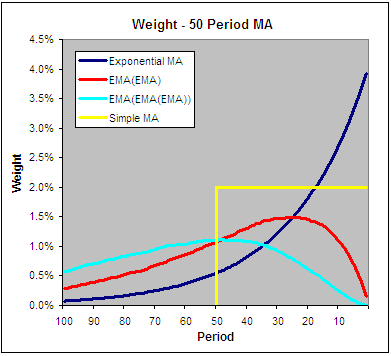
\includegraphics[width=0.9\textwidth]{graphics/chapter2/fingrundlagen/wrong_dema_tema.png}
			\caption[Falsche Multiple Exponential Average Gewichtung]{Falsche Double und Triple Exponential Average Gewichtung}
			\label{fig:wrong_dema_tema}
	\end{minipage}\hspace{0.01\textwidth}	% Abstand zwischen den Bildern = 1% der Textbreite
	\begin{minipage}[b]{0.4\textwidth}
		\centering
 			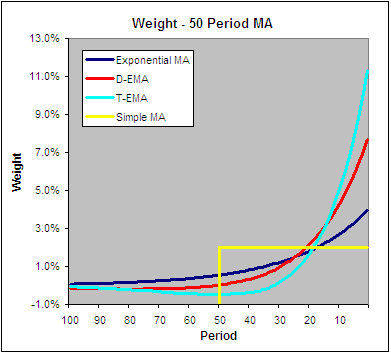
\includegraphics[width=0.9\textwidth]{graphics/chapter2/fingrundlagen/right_dema_tema.png}
			\caption[Richtige Multiple Exponential Average Gewichtung]{Richtige Double und Triple Exponential Average Gewichtung}
			\label{fig:right_dema_tema}
	\end{minipage}
\end{figure}

\cite{etf_hq_dema_tema}

\subsection{Unterst�tzung und Widerstand}

Die Kurse von Aktien unterliegen, wie bereits erw�hnt gewissen Trends, die entweder auf-, ab- oder auch seitw�rts verlaufen, wenn weder das eine, noch das andere klar feststellbar ist. Bei steigenden Kursen erreichen diese irgendwann ein Level, bei dem der Preis nicht mehr als billig angesehen wird und der Kurs dreht um. Der Trend verliert also seine Nachhaltigkeit. Dieses Level wird als \emph{Widerstand} oder \emph{Resistance} bezeichnet, da dieser nur schwer �berwunden wird. Sinkt der Kurs eine Weile wieder und sonstige Bewertungskriterien des Handelsgutes haben sich nicht signifikant ver�ndert, erreicht der Kurs einen Punkt, bei dem er wieder interessant f�r etwaige K�ufer wird. Diese Schwelle wird als \emph{Unterst�tzung} oder \emph{Support} bezeichnet. Am Beispiel von Microsoft kann diese Funktion in der Grafik \ref{fig:msft_sup_res} �ber einen l�ngeren Zeitraum beobachtet werden.\\
	Diese beiden Schwellen sind tempor�re Hilfsmittel und lassen Wendepunkte erahnen. Bei Durchbruch eines Levels, kann hingegen mit einer Fortsetzung dieses Trends gerechnet werden und ggf. wird ein alter Widerstand zur Unterst�tzung. \cite{godmode_supp_res} Das Chart \ref{fig:payx_sup_res} von Paychex Inc. veranschaulicht diesen Wechsel von Unterst�tzungs- zu Widerstands- und wieder zur�ck zu Unterst�tzungslevel.

\begin{figure}
	\centering
		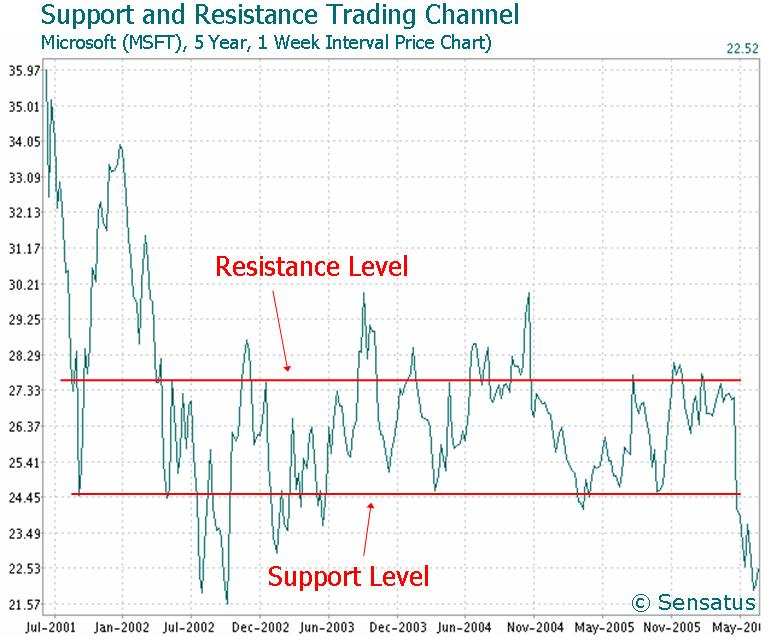
\includegraphics[width=0.8\textwidth]{graphics/chapter2/msft_sup_res.JPG}
	\caption[Microsoft Support Resistance]{Microsoft 5-Jahres-Chart mit 1-Wochen-Intervallen und eingezeichneten Support- und Resistance-Level}
	\label{fig:msft_sup_res}
\end{figure}

\begin{figure}
	\centering
		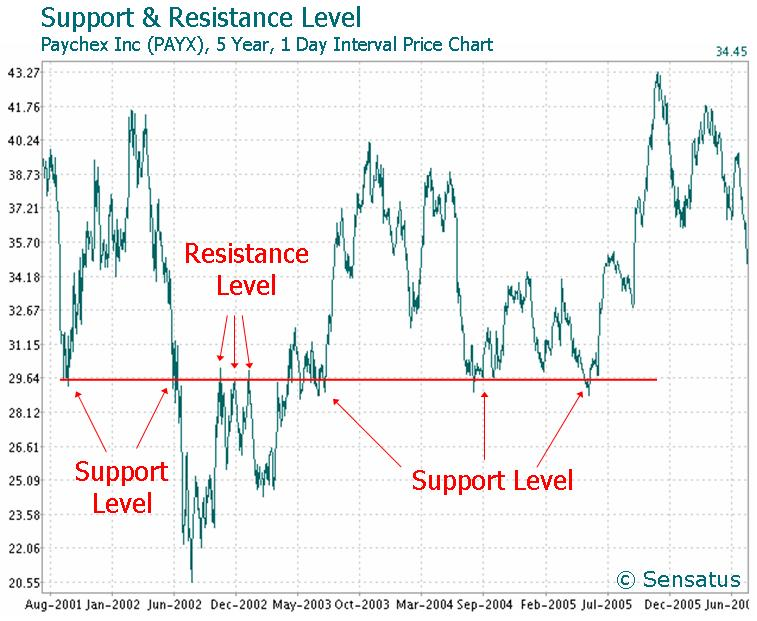
\includegraphics[width=0.8\textwidth]{graphics/chapter2/payx_sup_res.JPG}
	\caption[Paychex Inc. Support Resistance]{Paychex Inc. 5-Jahres-Chart mit 1-Wochen-Intervallen; Level wechselt zwischen Support- und Restistance-Funktion}
	\label{fig:payx_sup_res}
\end{figure}

\subsubsection{Prozentb�nder}

Prozentb�nder sind eine andere M�glichkeit Nachhaltigkeit bzw. �berkauft- oder �berverkauft-Level festzustellen. Dazu wird ein \gls{ma} um einen festgelegten Prozentwert nach unten und oben verschoben, so dass ein Kanal bzw. ein Band entsteht, in dem der Kurs die meiste Zeit verl�uft. Wenn der Kurs �ber dem oberen Band notiert, wird dieser meist als �berkauft angesehen, da er im Vergleich zum Durchschnitt sehr schnell gestiegen ist. Um wie viel Prozent die B�nder nach oben und unten verschoben werden, h�ngt von der L�nge des \gls{ma} und somit dem Tradingzeitraum ab. Oft gebraucht werden 3\%-B�nder und eine 21-Tage-Linie oder 10\%-B�nder mit einem 40-Wochen-\gls{ma}.

\subsubsection{Bollinger B�nder}

Die Bollinger-B�nder, entwickelt von John Bollinger, sind ein �hnlicher Indikator, wie die Prozentb�nder. Es wird ebenso ein Bereich oberhalb und unterhalb des \gls{ma} aufgespannt, aber anstatt ihn einfach um einen fixen Prozentwert zu verschieben, wird die Durchschnittslinie um die \emph{Doppelte Standardabweichung}, die meist auf L�nge des \gls{ma} berechnet wird, nach oben und nach unten verschoben.\\
	Dabei dienen die B�nder meist als Kursziele, so dass beim ansteigen des Kurses vom unteren Bollinger-Band, das obere als Ziel angenommen wird. Der Durchmesser der B�nder zeigt die Volatilit�t des Kurses an, da bei geringer Volatilit�t die Standardabweichung ebenfalls sinkt, ergo werden die B�nder schm�ler.

\subsubsection{Aroon}

Der 1995 von Tushar S. Chande entwickelte Aroon ist ein zweigeteilter Trendindikator, der zwar nicht die St�rke eines Trends anzeigt, aber gut die Marktlage erfasst. So kann beispielsweise erkannt werden, ob es sich um eine Trend- oder eher um eine Seitw�rtsphase handelt. Die Signale sind dabei sehr einfach abzulesen und fluktuieren sehr wenig, da die Trendst�rke, wie bereits erw�hnt, nicht direkt erfasst wird, sondern nur zeitlich, sodass ein Verlust des Momentums feststellbar wird. Die St�rke des Indikators ist es, schnell einen Trendwechsel bzw. Marktzustandswandel anzuzeigen. Die klaren Signale eignen sich au�erdem gut f�r algorithmische Handelssysteme, wenn die St�rke des Trends durch eine andere Komponente erfasst wird.\\
	Aroon besteht aus einem Aroon-Up und einem Aroon-Down, die jeweils die vergange Zeit zu einem Kursextrem anzeigen und zwischen 0 und 100 variieren. Bei einem 14-Tage-Aroon hat der Aroon-Up bei einem aktuellen 14-Tages-Hoch einen Wert von 100.\\
	Zur Interpretation ist eine Signallinie sehr wichtig, die von Chande bei einem Wert von 75 angesetzt wurde, aus anderen Quellen sind auch Werte um die 90 zu finden. Liegt der Aroon-Up �ber dem Aroon-Down und steigt zus�tzlich noch �ber die Signallinie ist dies als Aufw�rtstrend zu identifizieren. Da der Indikator h�ufig kurzfristig unter die Signallinie f�llt (s. \ref{fig:aroon}), ist es noch nicht ratsam zu diesem Zeitpunkt die Positionen zu liquidieren, sondern noch zu warten bis sich die Up- und Down-Linien ebenfalls �berkreuzen.\\
	Ein Seitw�rtstrend wird angezeigt, wenn sich Aroon-Up und -Down unter der Signallinie befinden, was bei liquiden Positionen nur kurzfristig auftritt. \cite{charttec_aroon}\\

\begin{figure}
	\centering
		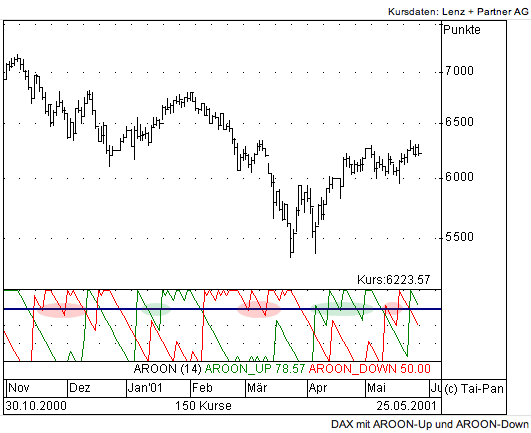
\includegraphics[width=0.8\textwidth]{graphics/chapter2/fingrundlagen/aroon.png}
	\caption[Aroon Indicator]{14-Tage Aroon �ber 7 Monate des DAX-Kurses}
	\label{fig:aroon}
\end{figure}

Die Berechnung des Aroon-Up und Aroon-Down ist mit den folgenden Formeln beschrieben. Wobei $high_{n+1}$ in \ref{Aroon-Up} die Zeit seit dem h�chstem Hoch innerhalb von $n+1$ Perioden und $low_{n+1}$ in \ref{Aroon-Down} die Zeit seit dem tiefstem Tief innerhalb von $n+1$ Perioden bezeichnet.

\begin{equation}
	\label{Aroon-Up}
	\frac{n-high_{n+1}}{n}*100
\end{equation}

\begin{equation}
	\label{Aroon-Down}
	\frac{n-low_{n+1}}{n}*100
\end{equation}

\subsection{Handelsstrategien}

In diesem Punkt sollen verbreitete Handelsstrategien erl�utert werden, um einerseits potentiell zu testende Algorithmen festzustellen und andererseits eine Grundlage f�r Weiterentwicklung und Kombinationsm�glichkeiten aufzuzeigen.

\subsubsection{Preiskreuzung des Gleitenden Durchschnitts}

Eine simples Tradingmodell, dass von einigen Tradern verwendet wird, basiert auf einer einfachen �berkreuzung eines \gls{ma} �ber den Preis. Es wird dabei angenommen, dass wenn der Preis �ber den \gls{ma} steigt, ein Aufw�rtstrend eingesetzt hat, da der Kurs begonnen hat schneller als der l�ngere Durchschnitt zu steigen. Umgekehrt wird angenommen, dass bei einem Abfall des Kurses unter den \gls{ma} ein Abw�rtstrend folg und daher wird ein short-Signal generiert. Eine zus�tzliche Sicherheit ist gegeben, wenn der \gls{ma} selbst in erwartete Kursrichtung dreht.\\
	Dieser simple Algorithmus hat einige Nachteile. Es ist zu jedem Zeitpunkt ein Signal gegeben, was bedeutet dass immer entweder eine long- oder eine short-Position gehalten wird. Au�erdem verliert diese Strategie bei langen \glspl{ma} nach der Trendumkehr wieder viel des Gewinns, da das Gegensignal erst sp�t generiert wird. Kurze \glspl{ma} erzeugen oft Fehlsignale.

\subsubsection{Verwendung Mehrerer Gleitender Durchschnitte}

Eine h�ufig verwendete Variante zur Signalgenerierung mit \glspl{ma} wird \emph{Double Crossover Method} genannt. Dabei kommen 2 unterschiedlich lange \glspl{ma} zum Einsatz, wobei ein Signal erzeugt wird wenn sich beide schneiden. Kreuzt der kurze \gls{ma} den l�ngeren entsteht ein Kaufsignal, auch \emph{Golden Cross} genannt, und vice versa. Diese Variante erzeugt weniger Fehlssignale, als die direkte Verwendung des Preises, hinkt dem Markt daf�r aber auch st�rker hinterher. Die L�nge der Durchschnitte h�ngt wie immer sowohl vom Handelszeitraum und der gew�nschten Signalanzahl, als auch vom Markt ab.\\
\\
Dieses System kann noch um einen weiteren \gls{ma} raffiniert werden. Der Einsatz dreier Durchschnitte, oder \emph{Triple Crossover Method} verfeinert die Art des Signals. Ein vollst�ndiges Kaufsignal entsteht sobald der kurze �ber dem mittleren, und jener wiederum �ber dem langen \gls{ma} notiert. Eine umgekehrte Anordung ist als Verkaufssignal anzusehen.\\
	Beginnt der kurze Trendfolger �ber den mittleren und anschlie�end auch �ber den langen zu steigen, ist dies als vorbereitendes Kaufsignal zu interpretieren. Wenn der mittlere anschlie�end den langen auch noch von unten schneidet ist das Signal vollst�ndig.\\
	Auf diese Art kann beispielsweise bei unklaren Signalen eine Neutralstellung (i.e. keine Aktien im Portfolio) eingenommen werden oder die Market-Exposure (i.e. Anzahl der Aktien) reduziert werden.\\
	Normalerweise werden f�r solche Systeme \glspl{sma} verwendet, wobei aber besonders bei einem Double Crossover System die Anwendung eines \gls{ema} oder sogar 

\subsubsection{Moving Average Convergence/Divergence}


\clearpage
\section{Voruntersuchung}

\subsection{IST-Erhebung}

Es wird bereits ein Gro�teil des Kapitals in Wertpapieren algorithmisch verwaltet. Daher existiert eine Unmenge an Wissen �ber den Aufbau
von B�rsenalgorithmen und die Anwendung von Indikatoren zur Einsch�tzung von zuk�nftigen Kurswerten. Die meisten dieser Algorithmen basieren auf technischer
Analyse und den simplen Algorithmen die diese mit sich bringt.Bekannte Vertreter davon sind zum Beispiel der MACD und der CCI.
Die meisten Algorithmen benutzen au�erdem eine Zusammensetzung aus verschiedenen \glspl{ma}, um die zu Grunde liegenden Handelsentscheidungen zu treffen.
Aufgrund dieses umfangreichen Wissens ist es m�glich weitere M�glichkeiten zu erforschen und noch besser und sinnvoller handelnde maschinelle Helfer zu kreieren.\\
\\
Ein Problem der aktuellen Situation ist allerdings, das schlechte bzw. umst�ndliche Testing dieser Algorithmen, da wenig Software existiert, die
verifizieren kann ob ein Algorithmus in bestimmten Marktphasen bestimmte Leistungen erbringt. Au�erdem ist es momentan ziemlich kompliziert sich einfach
die gesamte Performance eines solchen Handelsalgorithmus anzusehen. Es gibt hierf�r aber sowohl Gratisquellen, als auch kommerzielle Produkte, von denen man
historische Daten zum Backtesting dar Algorithmen beziehen kann. Das Projektteam von Noctua besitzt bereits ca. 3.9 Gb an historischen B�rsenkursen von
e-Signal \footnote{http://www.esignal.com/default.aspx?tc=} und nahezu unbegrenzten Zugriff auf weitere Daten vom selben Anbieter.
Dadurch ist es ihm m�glich Algorithmen �ber ein weites Spektrum von Marktphasen und -zust�nden hinweg zu testen und die Performance verschiedener Algorithmen in unterschiedlichen Situationen akkurat festzustellen. Dies ist besonders wichtig, da Algorithmen die in der nahen Vergangenheit guten Entscheidungen trafen, meist weiterhin sehr erfolgreich handeln und den Anleger m�glicherweise mit einem Kapitalzuwachs belohnen.

\subsection{IST-Zustand}

Aufgrund der riesingen Industrie die diesem Projekt zu Grunde liegt gibt es nat�rlich bereits eine Vielzahl an Konkurrenzprodukten auf dem Markt. Einige davon spezialisieren sich auf das Backtesting bzw. die Bereitstellung einer Plattform zur Entwicklung von Algorithmen. Andere sind eher propriet�rer Natur und versuchen lediglich durch Korruption der Konkurrenz, selbst den wirtschaftlich rentabelsten Algorithmus zu betreiben. Doch alle haben ihre Vor- und Nachteile. Daher finden sich auch immer wieder neue Nieschen f�r Neueinsteiger am Markt, die durch ausgekl�gekte Algorithmen viel erreichen k�nnen. Im folgenden werden nun die bekanntesten dieser Konkurrenzprodukte berschrieben.

\subsubsection{MetaTrader 5}

Hierbei handelt es sich um ein ziemlich umfangreiches, ein wenig �lteres Produkt, dass sowohl Aktien- als auch Forex-Daten anbietet. MetaTrader 5 ist die neue verbesserte Version von Metatrader 4 und bietet neben den alten Funktionen, Neuerungen wie die Einbindung von News. Au�erdem bietet der MetaTrader ein weites Spektrum an Indikatoren, die einfach in den laufenden Betrieb eingebunden werden k�nnen. Die Oberfl�che des MetaTraders sieht in etwa aus, wie in Abbildung \ref{fig:metatrader5_overview} dargestellt.

\begin{figure}
	\centering
		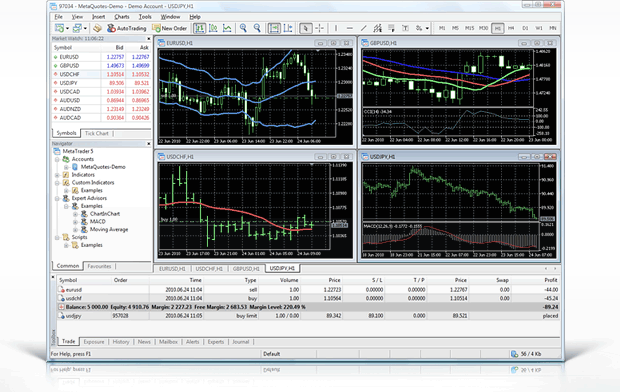
\includegraphics{graphics/chapter2/metatrader5_overview.png}
	\caption{MetaTrader 5 Oberfl�che}
	\label{fig:metatrader5_overview}
\end{figure}

\begin{figure}
	\centering
		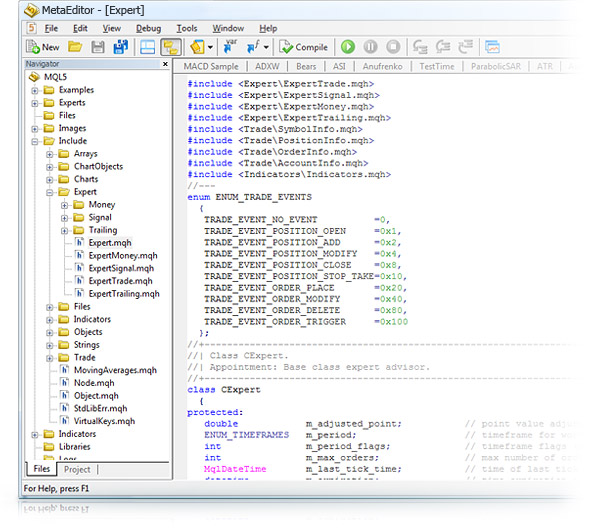
\includegraphics{graphics/chapter2/metaeditor_robot_modification.jpg}
	\caption{MetaTrader 5 IDE-Oberfl�che}
	\label{fig:metaeditor_robot_modification.jpg}
\end{figure}

Doch das gr��te Feature des MetaTraders ist die eingebaute IDE(siehe Abbildung \ref{fig:metaeditor_robot_modification.jpg}), die es mittels einer eigenen MetaTrader-spezifischen Sprache, der \gls{mql5}, erm�glicht eigene Algorithmen zu programmieren und diese dann auch direkt in den laufenden Betrieb zu �bernehmen. Der MetaTrader bietet sogar einen j�hrlichen Wettberewerb an, bei dem er jedes Jahr einen der besten Algorithmen zum Sieger k�rt. Die neue Sprache \gls{mql5} ist sogar ebenfalls noch weiter gegen�ber der MQL4 verbessert. Dies f�hrt uns allerdings auch schon zum Problem beim MetaTrader 5, da nur ein geringer Teil der Software Entwickler gewillt ist, wirklich extra eine neue Programmiersprache zu lernen, nur einen Algorithmus entwicklen und testen zu k�nnen, der dann selbst wiederum auch an den MetaTrader gebunden ist nich in den normalen operativen Betrieb portiert werden kann. Au�erdem ist der MetaTrader eines der sehr wenigen Produkte am Markt, die es Nutzern wirklich erm�glicht einen Algorithmus zu entwickeln und zu testen ohne die gesamte struktur rundherum zuerst aufzubauen. Daher ist es n�tig diesem Mangel Abhilfe zu schaffen und eine \gls{bts} zu entwicklen, die genau dies erm�glicht und ohne den Nutzer dabei an das Unternehmen in dem er seinen Algorithmus testet zu binden.

\clearpage
\chapter{Produktfunktionen} \label{chapter:produktfunktionen}

\section{Must-Have}

/F010/\\
\textit{Vergangene Marktzust�nde bestimmen}

\begin{center}

\begin{tabular}{ | l | p{10cm} |}
\hline 
Beschreibung & Es sollen historische Marktzust�nde (innerhalb der letzten Jahre), auf transparenten
Aktienm�rkten, f�r die ein ausreichender Datenbestand vorhanden ist, automatisch bestimmt
werden. Sollten sich verschiedene gro�e M�rkte entgegen Erwartung entsprechend
unterschiedlich verhalten, dass diese keiner einheitlichen Analyse unterzogen werden k�nnen,
soll prim�r der US-amerikanische Aktienmarkt untersucht werden. Hierbei handelt es sich um
eine Gruppierung von Zeitabschnitten nach gemeinsamen Kriterien.\\  \hline
Aufwand & Hoch \\ \hline
Nutzen & Hoch \\ \hline
Ziel & Ermittelung von Klassen f�r Marktzust�nde. \\ \hline
Vorbedingungen & - \\ \hline
Nachbedingungen & - \\ \hline

\end{tabular}

\end{center}

/F020/\\
\textit{Aktuellen Marktzustand bestimmen}

\begin{center}

\begin{tabular}{ | l | p{10cm} |}
\hline 
Beschreibung & Dabei soll darauf geachtet werden, dass f�r eine fr�he Erkennung m�glicherweise nur ein Teil
der Daten vorhanden ist, die f�r die historische Analyse herangezogen werden.\\  \hline
Aufwand & Mittel \\ \hline
Nutzen & Hoch \\ \hline
Ziel & Zuordnung des aktuellen Marktzustandes zu einem bereits Bekannten. \\ \hline
Vorbedingungen & /F010/ Vergangene Marktzust�nde bestimmen \\ \hline
Nachbedingungen & - \\ \hline

\end{tabular}

\end{center}

/F110/\\
\textit{Trends erkennen}

\begin{center}

\begin{tabular}{ | l | p{10cm} |}
\hline 
Beschreibung & Durch \glspl{ma} soll es m�glich sein Trends in Aktienkursen zu identifizieren. Dazu
kommen verschiedene Crossover-Verfahren (double- / triple-crossover) oder Indikatoren, wie
der MACD (Moving Average Convergence Divergence) in Frage. Es soll eine statistisch
m�glichst profitable Variante hierf�r gefunden werden, die aufscheinende nachhaltige Trends
m�glichst g�nstig erkennt.\\  \hline
Aufwand & Hoch \\ \hline
Nutzen & Hoch \\ \hline
Ziel & Fr�hzeitige m�glichst profitable Erkennung von Trends. \\ \hline
Vorbedingungen & - \\ \hline
Nachbedingungen & - \\ \hline

\end{tabular}

\end{center}

/F120/\\
\textit{\gls{ma}-Dauer bestimmen}

\begin{center}

\begin{tabular}{ | l | p{10cm} |}
\hline 
Beschreibung & Je nachdem, wie lange ein Trend andauert, bedingt eine Trenderkennung andere \gls{ma}(-Paare)
mit unterschiedlichen Laufzeiten. Aus z.B. bew�hrten Wertepaaren oder adaptiven Methoden sollen
automatisch die optimalen Laufzeiten gew�hlt werden.\\  \hline
Aufwand & Niedrig \\ \hline
Nutzen & Mittel \\ \hline
Ziel & Erarbeitung eines optimalen Parametersatzes f�r ein \gls{ma}-Paar. \\ \hline
Vorbedingungen & - \\ \hline
Nachbedingungen & - \\ \hline

\end{tabular}

\end{center}

/F130/\\
\textit{An Marktzustand anpassen}

\begin{center}

\begin{tabular}{ | l | p{10cm} |}
\hline 
Beschreibung & Der Algorithmus soll sich durch Parameterver�nderung an den erkannten Marktzustand zur
Optimierung der Performance anpassen. Dies kann beispielsweise durch ver�ndern der \gls{ma}-Paare
oder durch Anpassung der Market Exposure und damit des Risikos erfolgen.
Dazu \textit{k�nnen} die Implikationen durch Nachforschung bekannt sein, woraufhin ein Modell
angewandt wird, m�ssen aber nicht, da auch induktiv aus den Implikationen gelernt werden
kann, wonach automatisch ein Modell entsteht. (\textit{Maschinelles Lernen}) Dabei werden f�r die
unterschiedlichen Markzust�nde verschiedene Parameters�tze durchprobiert.\\  \hline
Aufwand & Hoch \\ \hline
Nutzen & Hoch \\ \hline
Ziel & Anpassung der Hauptfunktionen des Algorithmus an den aktuellen Marktzustand. \\ \hline
Vorbedingungen & /F020/ Aktuellen Marktzustand bestimmen \\ \hline
Nachbedingungen & - \\ \hline

\end{tabular}

\end{center}

/F140/\\
\textit{Signale generieren}

\begin{center}

\begin{tabular}{ | l | p{10cm} |}
\hline 
Beschreibung & Signalgeben bei potentiellen Einstiegspunkten (long signal) und Ausstiegspunkten (short
signal).\\  \hline
Aufwand & Niedrig \\ \hline
Nutzen & Hoch \\ \hline
Ziel & R�ckgabe von Handelssignalen. \\ \hline
Vorbedingungen & /F110/ Trends erkennen, /F130/ An Marktzustand anpassen, /F120/ \gls{ma}-Dauer bestimmen \\ \hline
Nachbedingungen & /F160/ Signale filtern \\ \hline

\end{tabular}

\end{center}

/F150/\\
\textit{Trend-Nachhaltigkeit bestimmen}

\begin{center}

\begin{tabular}{ | l | p{10cm} |}
\hline 
Beschreibung & Durch geeignete Support- und Resistance-Indikatoren soll die Nachhaltigkeit eines Trends
bestimmt werden (beispielsweise Pivot Points, RSI, CCI oder MAs), um den Ausstiegspunkt zu
optimieren.\\  \hline
Aufwand & Mittel \\ \hline
Nutzen & Hoch \\ \hline
Ziel & Festellen der Nachhaltigkeit erkannter Trends. \\ \hline
Vorbedingungen & /F140 Signale generieren \\ \hline
Nachbedingungen & - \\ \hline

\end{tabular}

\end{center}

/F160/\\
\textit{Signale filtern}

\begin{center}

\begin{tabular}{ | l | p{10cm} |}
\hline 
Beschreibung & Zur Verminderung von unprofitablen, zu kurzen Trades sollen insbesondere Kaufsignale
gefiltert werden. Die Trenderkennung k�nnte des �fteren zu kurz anhaltende Trends
erkennen, indem beispielsweise ein MA-Crossover nur f�r kurze Zeit besteht. Durch das
Einf�hren eines Schwellenwertes (threshold), der �berschritten werden muss, oder eine
bestimmte Zeitspanne, die ein Signal �berdauern muss k�nnen zu kurze Trades vermindert
werden, wenn sich im Backtesting dadurch ein Vorteil herausgestellt hat.\\  \hline
Aufwand & Mittel \\ \hline
Nutzen & Hoch \\ \hline
Ziel & Filterung der unbrauchbaren Signale. \\ \hline
Vorbedingungen & /F140/ Signale generieren, /F150/ Trend-Nachhaltigkeit bestimmen \\ \hline
Nachbedingungen & - \\ \hline

\end{tabular}

\end{center}

/F210/\\
\textit{Performance berechnen}

\begin{center}

\begin{tabular}{ | l | p{10cm} |}
\hline 
Beschreibung & Die relative Performance eines Algorithmus soll in Prozent der Kapitalver�nderung berechnet
werden.\\  \hline
Aufwand & Mittel \\ \hline
Nutzen & Hoch \\ \hline
Ziel & Berechnung der relativen Performance eines Algorithmus \\ \hline
Vorbedingungen & - \\ \hline
Nachbedingungen & - \\ \hline

\end{tabular}

\end{center}

/F220/\\
\textit{Gewinn/Risiko-Verh�ltnis berechnen}

\begin{center}

\begin{tabular}{ | l | p{10cm} |}
\hline 
Beschreibung & Bestimmung des Risikos des Algorithmus (beispielsweise anhand der Volatilit�t) in
Verbindung mit der Performance (e.g. sharpe ratio).\\  \hline
Aufwand & Niedrig \\ \hline
Nutzen & Mittel \\ \hline
Ziel & Bestimmung des Gewinn/Risiko-Verh�ltnisses eines Algorithmus \\ \hline
Vorbedingungen & /F210/ Performance berechnen \\ \hline
Nachbedingungen & - \\ \hline

\end{tabular}

\end{center}
\clearpage
\section{Technische Machbarkeit}\label{section:Technische Machbarkeit}
\subsection{Variantenbildung}
Die \gls{bts} kann man in jeder erdenklichen Programmiersprache schreiben, allerdings ist es wichtig daran zu denken, dass das Programm einerseits effizient arbeiten soll und deswegen hardwarenahe rechnet, und andererseits hat das Projektteam mit manchen Programmiersprachen keinerlei Erfahrung.\\
Die allgemeine Funktionalit�t muss das lesen und schreiben von Dateien sein, aber auch das algorithmische Rechnen soll effizient funktionieren. F�r das Team kommen daher 3 M�glichkeiten in Frage: Eine L�sung in reinem C++, welches sehr hardwarenahe arbeitet, eine Mischung aus F\# und C\#, mit der eine paralelisierte Berechnung m�glich w�re, und eine Java-L�sung, bei der das Team die gr��te Erfahrung mitbringt. \\
Bei der Kombination agiert C\# als Handlungs- und Steuerkern und F\# als funktionale Programmiersprache, als Rechenkern und \"Mastermind\" der Applikation, welches die Entscheidungen trifft. Hierbei wird einerseits eine enorm hohe Arbeitsgeschwindigkeit erm�glicht, da die beiden Sprachen relativ hardwarenah agieren und andererseits besteht der nicht zu untersch�tzende Vorteil bzw. die M�glichkeit, den Rechenkern auf ein externes System outzusourcen, welches zum Beispiel enorme Rechenkapazit�ten aufweisen k�nnte und somit viel komplexere und effizientere Algorithmen in annehmbarer Zeit durchrechnen und abh�ngig davon mehr gewinnbringende Entscheidungen treffen k�nnte. Dabei sollte es auch bei sp�teren Erweiterungen des Programms zu keinem signifikanten Geschwindigkeitsabfall kommen.


\begin{center}

\begin{tabular}{ | c | p{2.6cm} | p{1.7cm} | p{0.5cm} |p{0.5cm}|p{0.5cm}|p{0.5cm}|p{0.7cm}|p{0.7cm}|}
\hline 
\multicolumn{2}{|p{1.5cm}|}{ }  & Gewicht\-ung & \multicolumn{2}{p{1.5cm}|}{\textbf{C++ R*G}} & \multicolumn{2}{p{1.5cm}|}{\textbf{Java R*G}} & \multicolumn{2}{|p{1.5cm}|}{\textbf{C/F R*G}}\\ \hline
\multirow{6}{*}{Einfachheit} & Aufwand Coding & 10\% & 3 & 30 & 1 & 10 & 2 & 20 \\ \cline{2-9}
& Bedinung/ Wartung & 6\% &3&9&2&6&1&3\\ \cline{2-9}
& Update &3\%&3&9&2&6&1&3\\ \cline{2-9}
& Integration &5\%&3&15&2&10&1&5\\  \cline{2-9}
& Kenntnisse &6\%&3&18&1&6&2&12\\ \cline{2-9}
& \textbf{Gesamt}&30\%&3&90&2&44&1&46\\ \hline
\multirow{5}{*}{Leistung}& �bertragungs-zeit &6\%&1&6&3&18&2&12\\ \cline{2-9}
& Absturz-sicherheit &5\%&1&5&2&10&3&15\\ \cline{2-9}
& Ressourcen-verbrauch &3\%&1&3&3&9&2&6\\ \cline{2-9}
& Datenumfang &1\%&1&1&3&3&2&2\\ \cline{2-9}
& \textbf{Gesamt} &15\%&1&15&3&50&2&35\\ \hline
\multirow{5}{*}{Kosten}& Lizenzen &10\%&1&10&1&10&&\\ \cline{2-9}
& Support &5\%&3&15&1&5&2&10\\ \cline{2-9}
& Betriebs-kosten &\%&&&&&&\\ \cline{2-9}
& Dokumen-tation &5\%&1&5&2&20&3&15\\ \cline{2-9}
& \textbf{Gesamt} &\%&&&&&&\\ \hline
\multirow{4}{*}{Dokumentation}& Verf�gbarkeit &10\%&3&30&2&20&1&10\\ \cline{2-9}
& Voll-st�ndigkeit &10\%&3&30&2&20&1&10\\ \cline{2-9}
& Qualit�t &10\%&2&20&1&10&1&10\\ \cline{2-9}
& \textbf{Gesamt} &30\%&3&80&2&50&1&30\\ \hline
\end{tabular}

\end{center} 

\begin{center}

\begin{tabular}{|l|r|p{0.8cm}|p{0.8cm}|p{0.8cm}|p{0.8cm}|p{0.8cm}|p{0.8cm}|} \hline
Kapitel&Gewichtung&\multicolumn{2}{p{1.8cm}|}{\textbf{C++}}&\multicolumn{2}{p{1.8cm}|}{\textbf{Java}}&\multicolumn{2}{p{1.8cm}|}{\textbf{C\#/F\#}}\\ \hline
Einfachheit&30\%&3&90&2&44&1&46 \\ \hline
Leistung&\%&&&&&& \\ \hline
Kosten&\%&&&&&& \\ \hline
Dokumentation&\%&&&&&& \\ \hline
\end{tabular}

\end{center}

\begin{center}
\begin{tabular}{|l|l|l|l|} \hline
Gesamtbewertung&&&\\ \hline
Endreihung &&&\\ \hline
\end{tabular}
\end{center}


\clearpage
% Wirtschaftliche Machbarkeit

\section{Wirtschaftliche Machbarkeit} \label{chapter:Wirtschaftliche Machbarkeit}

\subsection{Aufwandsabsch�tzung}

\subsection{Nutzen}

\subsection{Pr�fen der Risiken}
\subsubsection{Personenausfall}
Eintrittswahrscheinlichkeit:  gering \\
Auswirkungen:  								hoch   \\

In dem unerwarteten Fall, dass ein Teammitglied l�ngerfristig ausf�llt, muss es m�glich sein die Arbeitsaufgaben dementsprechend neu aufteilen zu k�nnen.
Folgende F�lle k�nnten auftreten:
\begin{itemize}
	\item Streit im Team
	\item Ausfall durch Krankheit oder Tod eines Teammitglieds
	\item Austritt eines Teammitglieds aus dem Projekt
	\item Der Auftraggeber k�nnte aufgrund von Unklarheiten den Projektabbruch initiieren 
	\item Es kann passieren, dass von Seite des Auftragsgebers pl�tzlich kein Interesse an der Umsetzung des Produktes mehr gegeben ist, und es dadurch zu extremem Zeitverzug kommt, was bis zum Abbruch f�hren kann
	\item Interessensverlusst eines Teammitglieds, und damit verbundene minderwertigere Arbeit 
\end{itemize}

Folgende pr�ventive Ma�nahmen werden eingef�hrt:
\begin{itemize}
	\item Regeln f�r den Umgang innerhalb des Projekts
	\item Ausreichendes Interesse jedes Mitglieds und keine leistungstechnische Probleme 
	\item Gutes Verh�ltnis mit den Auftraggebern
\end{itemize}

\subsubsection{Zeitliche Risiken}

Eintrittswahrscheinlichkeit:  gering \\
Auswirkungen:  								mittel \\

Die Aufwands- und Zeitsch�tzung basiert auf dem derzeitigen Lastenheft des Auftraggebers und stellt eine zeitgerechte Fertigstellung sicher. Sollten sich jedoch die Anforderungen des Kunden w�hrend des Projekts �ndern, so wird sich das mit gro�er Wahrscheinlichkeit verz�gernd auf den Fertigstellungstermin auswirken. Die mit dem Kunden vereinbarte Funktionsanalyse und die Meilensteine mit gemeinsam festgelegten Qualit�tskriterien sollten jedoch diesem Risiko entgegenwirken.

\subsubsection{Technische Risiken}
\label{subsection:Technische Risiken}
\textbf{Datenverlust}\\
Eintrittswahrscheinlichkeit:  gering \\
Auswirkungen:  								mittel \\

Aufgrund der nicht auszuschlie�enden Gefahr des Datenverlusts, muss daf�r gesorgt werden die Sicherheit der Daten, sowie auch die Verf�gbarkeit dieser zu garantieren. Dieses Problem wird mithilfe eines \gls{git} gel�st, durch diesen Server ist es m�glich die Versionen der Software immer zug�nglich zu machen und zus�tzlich die Daten auf den Computern der Projektmitgliedern zu speichern. \\ \\

\textbf{Hardwareausfall} \\
Eintrittswahrscheinlichkeit: gering \\
Auswirkung: mittel \\

Es kann ohne jede Vorwarnung immer und �berall ein Hardwareausfall passieren, dies kann selbst verschuldet, aber auch pl�tzlich passieren. Um mit einem solchen Ausfall zurecht zu kommen besitzt das Projektteam einen Ersatzlaptop um das gezielte Arbeiten auch nach dem 
Ausfall garantieren zu k�nnen. \\ \\

\textbf{Versionsverlust} \\
Eintrittswahrscheinlichkeit: sehr gering \\
Auswirkung: mittel \\

Bei den Versuchen mit dem Algorithmus wird andauernd etwas in der Datei ver�ndert. Bei dieser T�tigkeit kann es passieren das die Zusammenh�nge zwischen 1 oder mehreren Versionen des Algorithmus verloren gehen. Bei so einem Verlust kann auch das grundliegende Verst�ndnis f�r die jeweilige Version verloren gehen.\\
Folgende pr�ventive Ma�nahmen werden eingef�hrt:
\begin{itemize}
	\item Verwendung eines \gls{git}, f�r die automatische Versionierung
	\item Zwingende Benutzung der Bugtrackingsoftware
	\item Kommunikation im Team �ber die �nderungen am Algorithmus
\end{itemize}
\clearpage
\chapter{Projektorganisation} \label{chapter:Projektorganisation}

Der Grund daf�r, dass dieses Projekt ins Leben gerufen wurde, ist der Projektauftraggeber Herr Professor Mag. Hans Brabenetz und Herr Professor Dr. Helmut Vana. Der Projektleiter ist Peer Nagy und das Team besteht noch zus�tzlich aus zwei weiteren Entwicklern. Die anderen Projektteammitglieder sind Herr Gabriel Pawlowsky und Herr Josef Sochovsky.
\clearpage
% !TeX root = ../../Noctua_Diplomarbeit.tex

\section{Management Summary}
\label{section:management_summary}

Die Machbarkeitsstudie des Projektes NOCTUA behandelte die kritischen Punkte der Algorithmuskonzeption und -entwicklung und der \gls{bts}.\\
	Ein wichtiger Bestandteil waren Nachforschungen im Bereich der finanzwirtschaftlichen Grundlagen und der Technischen Analyse. Dabei wurden einige Trendfolgemechanismen und Oszillatoren beschrieben, um aus diesen und �hnlichen Mechanismen im Laufe des Projektes einen eigenen Algorithmus entwickeln zu k�nnen.\\
	Da es wichtig ist einen Algorithmus auch w�hrend der Laufzeit der \gls{bts} wechseln zu k�nnen, wird dieser in der Programmiersprache F\# entwickelt und als \gls{dll} gespeichert. Diese \gls{dll} kann einfach �ber eine \gls{gui} ausgew�hlt und f�r die aktuelle Berechnung herangezogen werden.\\
	Laut Aufwandssch�tzung entsteht ein Aufwand von insgesamt 480 h und Kosten in der H�he von \EUR{36.141}.
	
	\section{Versionierung} \label{section:versionierung}
\begin{center}

\begin{tabular}{ | l | p{2cm} | p{2cm} | p{2cm} | p{1.5cm} | p{2.8cm} | }
\hline 
\textbf{Version}�& \textbf{Autor} & \textbf{QS} & \textbf{Datum} & \textbf{Status} & \textbf{Kommentar} \\  \hline
0.1 & Sochovsky & Pawlowsky & 22.09.2012 & draft & Erstversion \\ \hline
0.2 & Pawlowsky & Nagy & 22.09.2012 & draft & Produkt\-funktionen\\ \hline
0.3 & Sochovsky & Pawlowsky & 23.09.2012 & draft & Technische Machbarkeit \\ \hline
0.4 & Sochovsky & Nagy & 24.09.2012 & draft & Nutzwert\-analyse\\ \hline
0.5 & Sochovsky & Pawlowsky & 26.09.2012 & draft & Wirtschaftliche Machbarkeit \\ \hline
0.6 & Nagy & Pawlowsky & 27.09.2012 & draft & Finanz\-wirtschaft\-liche Grundlagen \\ \hline
0.7 & Pawlowsky & Sochovsky & 28.09.2012 & draft & FPA \\ \hline
0.8 & Sochovsky & Nagy & 30.09.2012 & draft & Sollzustand \\ \hline
0.9 & Sochovsky & Nagy & 06.10.2012 & draft & Projekt\-organisation \\ \hline
1.0 & Pawlowsky & Sochovsky & 07.10.2012 & draft & Aufwands\-absch�tzung \\ \hline
1.1 & Nagy & Sochovsky & 15.10.2012 & draft & Einleitung \\ \hline
1.2 & Nagy & Pawlowsky & 17.10.2012 & Entwurf & Management Summary, Nutzen \\ \hline
\end{tabular}

\end{center}

%
% INCLUDES (\input) FOR CHAPTER 2 SUBFILES MOVED TO chapter2.tex
%\section{Voruntersuchung}

\subsection{IST-Erhebung}

Es wird bereits ein Gro�teil des Kapitals in Wertpapieren algorithmisch verwaltet. Daher existiert eine Unmenge an Wissen �ber den Aufbau
von B�rsenalgorithmen und die Anwendung von Indikatoren zur Einsch�tzung von zuk�nftigen Kurswerten. Die meisten dieser Algorithmen basieren auf technischer
Analyse und den simplen Algorithmen die diese mit sich bringt.Bekannte Vertreter davon sind zum Beispiel der MACD und der CCI.
Die meisten Algorithmen benutzen au�erdem eine Zusammensetzung aus verschiedenen \glspl{ma}, um die zu Grunde liegenden Handelsentscheidungen zu treffen.
Aufgrund dieses umfangreichen Wissens ist es m�glich weitere M�glichkeiten zu erforschen und noch besser und sinnvoller handelnde maschinelle Helfer zu kreieren.\\
\\
Ein Problem der aktuellen Situation ist allerdings, das schlechte bzw. umst�ndliche Testing dieser Algorithmen, da wenig Software existiert, die
verifizieren kann ob ein Algorithmus in bestimmten Marktphasen bestimmte Leistungen erbringt. Au�erdem ist es momentan ziemlich kompliziert sich einfach
die gesamte Performance eines solchen Handelsalgorithmus anzusehen. Es gibt hierf�r aber sowohl Gratisquellen, als auch kommerzielle Produkte, von denen man
historische Daten zum Backtesting dar Algorithmen beziehen kann. Das Projektteam von Noctua besitzt bereits ca. 3.9 Gb an historischen B�rsenkursen von
e-Signal \footnote{http://www.esignal.com/default.aspx?tc=} und nahezu unbegrenzten Zugriff auf weitere Daten vom selben Anbieter.
Dadurch ist es ihm m�glich Algorithmen �ber ein weites Spektrum von Marktphasen und -zust�nden hinweg zu testen und die Performance verschiedener Algorithmen in unterschiedlichen Situationen akkurat festzustellen. Dies ist besonders wichtig, da Algorithmen die in der nahen Vergangenheit guten Entscheidungen trafen, meist weiterhin sehr erfolgreich handeln und den Anleger m�glicherweise mit einem Kapitalzuwachs belohnen.

\subsection{IST-Zustand}

Aufgrund der riesingen Industrie die diesem Projekt zu Grunde liegt gibt es nat�rlich bereits eine Vielzahl an Konkurrenzprodukten auf dem Markt. Einige davon spezialisieren sich auf das Backtesting bzw. die Bereitstellung einer Plattform zur Entwicklung von Algorithmen. Andere sind eher propriet�rer Natur und versuchen lediglich durch Korruption der Konkurrenz, selbst den wirtschaftlich rentabelsten Algorithmus zu betreiben. Doch alle haben ihre Vor- und Nachteile. Daher finden sich auch immer wieder neue Nieschen f�r Neueinsteiger am Markt, die durch ausgekl�gekte Algorithmen viel erreichen k�nnen. Im folgenden werden nun die bekanntesten dieser Konkurrenzprodukte berschrieben.

\subsubsection{MetaTrader 5}

Hierbei handelt es sich um ein ziemlich umfangreiches, ein wenig �lteres Produkt, dass sowohl Aktien- als auch Forex-Daten anbietet. MetaTrader 5 ist die neue verbesserte Version von Metatrader 4 und bietet neben den alten Funktionen, Neuerungen wie die Einbindung von News. Au�erdem bietet der MetaTrader ein weites Spektrum an Indikatoren, die einfach in den laufenden Betrieb eingebunden werden k�nnen. Die Oberfl�che des MetaTraders sieht in etwa aus, wie in Abbildung \ref{fig:metatrader5_overview} dargestellt.

\begin{figure}
	\centering
		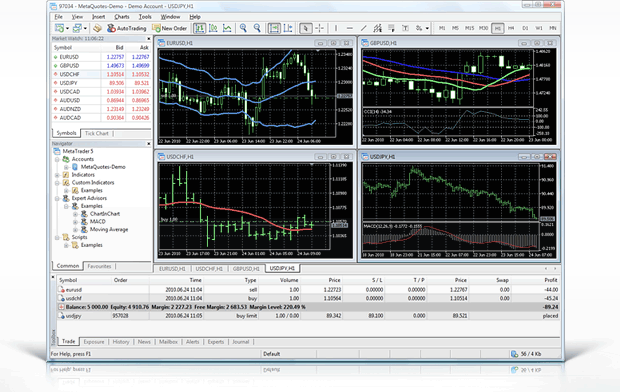
\includegraphics{graphics/chapter2/metatrader5_overview.png}
	\caption{MetaTrader 5 Oberfl�che}
	\label{fig:metatrader5_overview}
\end{figure}

\begin{figure}
	\centering
		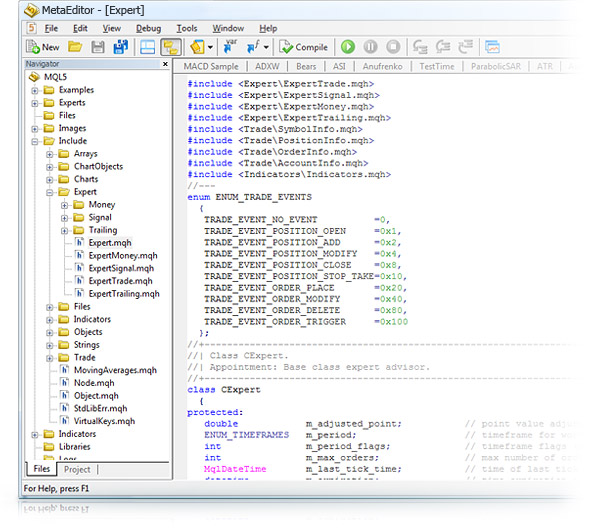
\includegraphics{graphics/chapter2/metaeditor_robot_modification.jpg}
	\caption{MetaTrader 5 IDE-Oberfl�che}
	\label{fig:metaeditor_robot_modification.jpg}
\end{figure}

Doch das gr��te Feature des MetaTraders ist die eingebaute IDE(siehe Abbildung \ref{fig:metaeditor_robot_modification.jpg}), die es mittels einer eigenen MetaTrader-spezifischen Sprache, der \gls{mql5}, erm�glicht eigene Algorithmen zu programmieren und diese dann auch direkt in den laufenden Betrieb zu �bernehmen. Der MetaTrader bietet sogar einen j�hrlichen Wettberewerb an, bei dem er jedes Jahr einen der besten Algorithmen zum Sieger k�rt. Die neue Sprache \gls{mql5} ist sogar ebenfalls noch weiter gegen�ber der MQL4 verbessert. Dies f�hrt uns allerdings auch schon zum Problem beim MetaTrader 5, da nur ein geringer Teil der Software Entwickler gewillt ist, wirklich extra eine neue Programmiersprache zu lernen, nur einen Algorithmus entwicklen und testen zu k�nnen, der dann selbst wiederum auch an den MetaTrader gebunden ist nich in den normalen operativen Betrieb portiert werden kann. Au�erdem ist der MetaTrader eines der sehr wenigen Produkte am Markt, die es Nutzern wirklich erm�glicht einen Algorithmus zu entwickeln und zu testen ohne die gesamte struktur rundherum zuerst aufzubauen. Daher ist es n�tig diesem Mangel Abhilfe zu schaffen und eine \gls{bts} zu entwicklen, die genau dies erm�glicht und ohne den Nutzer dabei an das Unternehmen in dem er seinen Algorithmus testet zu binden.
%
%\chapter{Produktfunktionen} \label{chapter:produktfunktionen}

\section{Must-Have}

/F010/\\
\textit{Vergangene Marktzust�nde bestimmen}

\begin{center}

\begin{tabular}{ | l | p{10cm} |}
\hline 
Beschreibung & Es sollen historische Marktzust�nde (innerhalb der letzten Jahre), auf transparenten
Aktienm�rkten, f�r die ein ausreichender Datenbestand vorhanden ist, automatisch bestimmt
werden. Sollten sich verschiedene gro�e M�rkte entgegen Erwartung entsprechend
unterschiedlich verhalten, dass diese keiner einheitlichen Analyse unterzogen werden k�nnen,
soll prim�r der US-amerikanische Aktienmarkt untersucht werden. Hierbei handelt es sich um
eine Gruppierung von Zeitabschnitten nach gemeinsamen Kriterien.\\  \hline
Aufwand & Hoch \\ \hline
Nutzen & Hoch \\ \hline
Ziel & Ermittelung von Klassen f�r Marktzust�nde. \\ \hline
Vorbedingungen & - \\ \hline
Nachbedingungen & - \\ \hline

\end{tabular}

\end{center}

/F020/\\
\textit{Aktuellen Marktzustand bestimmen}

\begin{center}

\begin{tabular}{ | l | p{10cm} |}
\hline 
Beschreibung & Dabei soll darauf geachtet werden, dass f�r eine fr�he Erkennung m�glicherweise nur ein Teil
der Daten vorhanden ist, die f�r die historische Analyse herangezogen werden.\\  \hline
Aufwand & Mittel \\ \hline
Nutzen & Hoch \\ \hline
Ziel & Zuordnung des aktuellen Marktzustandes zu einem bereits Bekannten. \\ \hline
Vorbedingungen & /F010/ Vergangene Marktzust�nde bestimmen \\ \hline
Nachbedingungen & - \\ \hline

\end{tabular}

\end{center}

/F110/\\
\textit{Trends erkennen}

\begin{center}

\begin{tabular}{ | l | p{10cm} |}
\hline 
Beschreibung & Durch \glspl{ma} soll es m�glich sein Trends in Aktienkursen zu identifizieren. Dazu
kommen verschiedene Crossover-Verfahren (double- / triple-crossover) oder Indikatoren, wie
der MACD (Moving Average Convergence Divergence) in Frage. Es soll eine statistisch
m�glichst profitable Variante hierf�r gefunden werden, die aufscheinende nachhaltige Trends
m�glichst g�nstig erkennt.\\  \hline
Aufwand & Hoch \\ \hline
Nutzen & Hoch \\ \hline
Ziel & Fr�hzeitige m�glichst profitable Erkennung von Trends. \\ \hline
Vorbedingungen & - \\ \hline
Nachbedingungen & - \\ \hline

\end{tabular}

\end{center}

/F120/\\
\textit{\gls{ma}-Dauer bestimmen}

\begin{center}

\begin{tabular}{ | l | p{10cm} |}
\hline 
Beschreibung & Je nachdem, wie lange ein Trend andauert, bedingt eine Trenderkennung andere \gls{ma}(-Paare)
mit unterschiedlichen Laufzeiten. Aus z.B. bew�hrten Wertepaaren oder adaptiven Methoden sollen
automatisch die optimalen Laufzeiten gew�hlt werden.\\  \hline
Aufwand & Niedrig \\ \hline
Nutzen & Mittel \\ \hline
Ziel & Erarbeitung eines optimalen Parametersatzes f�r ein \gls{ma}-Paar. \\ \hline
Vorbedingungen & - \\ \hline
Nachbedingungen & - \\ \hline

\end{tabular}

\end{center}

/F130/\\
\textit{An Marktzustand anpassen}

\begin{center}

\begin{tabular}{ | l | p{10cm} |}
\hline 
Beschreibung & Der Algorithmus soll sich durch Parameterver�nderung an den erkannten Marktzustand zur
Optimierung der Performance anpassen. Dies kann beispielsweise durch ver�ndern der \gls{ma}-Paare
oder durch Anpassung der Market Exposure und damit des Risikos erfolgen.
Dazu \textit{k�nnen} die Implikationen durch Nachforschung bekannt sein, woraufhin ein Modell
angewandt wird, m�ssen aber nicht, da auch induktiv aus den Implikationen gelernt werden
kann, wonach automatisch ein Modell entsteht. (\textit{Maschinelles Lernen}) Dabei werden f�r die
unterschiedlichen Markzust�nde verschiedene Parameters�tze durchprobiert.\\  \hline
Aufwand & Hoch \\ \hline
Nutzen & Hoch \\ \hline
Ziel & Anpassung der Hauptfunktionen des Algorithmus an den aktuellen Marktzustand. \\ \hline
Vorbedingungen & /F020/ Aktuellen Marktzustand bestimmen \\ \hline
Nachbedingungen & - \\ \hline

\end{tabular}

\end{center}

/F140/\\
\textit{Signale generieren}

\begin{center}

\begin{tabular}{ | l | p{10cm} |}
\hline 
Beschreibung & Signalgeben bei potentiellen Einstiegspunkten (long signal) und Ausstiegspunkten (short
signal).\\  \hline
Aufwand & Niedrig \\ \hline
Nutzen & Hoch \\ \hline
Ziel & R�ckgabe von Handelssignalen. \\ \hline
Vorbedingungen & /F110/ Trends erkennen, /F130/ An Marktzustand anpassen, /F120/ \gls{ma}-Dauer bestimmen \\ \hline
Nachbedingungen & /F160/ Signale filtern \\ \hline

\end{tabular}

\end{center}

/F150/\\
\textit{Trend-Nachhaltigkeit bestimmen}

\begin{center}

\begin{tabular}{ | l | p{10cm} |}
\hline 
Beschreibung & Durch geeignete Support- und Resistance-Indikatoren soll die Nachhaltigkeit eines Trends
bestimmt werden (beispielsweise Pivot Points, RSI, CCI oder MAs), um den Ausstiegspunkt zu
optimieren.\\  \hline
Aufwand & Mittel \\ \hline
Nutzen & Hoch \\ \hline
Ziel & Festellen der Nachhaltigkeit erkannter Trends. \\ \hline
Vorbedingungen & /F140 Signale generieren \\ \hline
Nachbedingungen & - \\ \hline

\end{tabular}

\end{center}

/F160/\\
\textit{Signale filtern}

\begin{center}

\begin{tabular}{ | l | p{10cm} |}
\hline 
Beschreibung & Zur Verminderung von unprofitablen, zu kurzen Trades sollen insbesondere Kaufsignale
gefiltert werden. Die Trenderkennung k�nnte des �fteren zu kurz anhaltende Trends
erkennen, indem beispielsweise ein MA-Crossover nur f�r kurze Zeit besteht. Durch das
Einf�hren eines Schwellenwertes (threshold), der �berschritten werden muss, oder eine
bestimmte Zeitspanne, die ein Signal �berdauern muss k�nnen zu kurze Trades vermindert
werden, wenn sich im Backtesting dadurch ein Vorteil herausgestellt hat.\\  \hline
Aufwand & Mittel \\ \hline
Nutzen & Hoch \\ \hline
Ziel & Filterung der unbrauchbaren Signale. \\ \hline
Vorbedingungen & /F140/ Signale generieren, /F150/ Trend-Nachhaltigkeit bestimmen \\ \hline
Nachbedingungen & - \\ \hline

\end{tabular}

\end{center}

/F210/\\
\textit{Performance berechnen}

\begin{center}

\begin{tabular}{ | l | p{10cm} |}
\hline 
Beschreibung & Die relative Performance eines Algorithmus soll in Prozent der Kapitalver�nderung berechnet
werden.\\  \hline
Aufwand & Mittel \\ \hline
Nutzen & Hoch \\ \hline
Ziel & Berechnung der relativen Performance eines Algorithmus \\ \hline
Vorbedingungen & - \\ \hline
Nachbedingungen & - \\ \hline

\end{tabular}

\end{center}

/F220/\\
\textit{Gewinn/Risiko-Verh�ltnis berechnen}

\begin{center}

\begin{tabular}{ | l | p{10cm} |}
\hline 
Beschreibung & Bestimmung des Risikos des Algorithmus (beispielsweise anhand der Volatilit�t) in
Verbindung mit der Performance (e.g. sharpe ratio).\\  \hline
Aufwand & Niedrig \\ \hline
Nutzen & Mittel \\ \hline
Ziel & Bestimmung des Gewinn/Risiko-Verh�ltnisses eines Algorithmus \\ \hline
Vorbedingungen & /F210/ Performance berechnen \\ \hline
Nachbedingungen & - \\ \hline

\end{tabular}

\end{center}%
%\section{Technische Machbarkeit}\label{section:Technische Machbarkeit}
\subsection{Variantenbildung}
Die \gls{bts} kann man in jeder erdenklichen Programmiersprache schreiben, allerdings ist es wichtig daran zu denken, dass das Programm einerseits effizient arbeiten soll und deswegen hardwarenahe rechnet, und andererseits hat das Projektteam mit manchen Programmiersprachen keinerlei Erfahrung.\\
Die allgemeine Funktionalit�t muss das lesen und schreiben von Dateien sein, aber auch das algorithmische Rechnen soll effizient funktionieren. F�r das Team kommen daher 3 M�glichkeiten in Frage: Eine L�sung in reinem C++, welches sehr hardwarenahe arbeitet, eine Mischung aus F\# und C\#, mit der eine paralelisierte Berechnung m�glich w�re, und eine Java-L�sung, bei der das Team die gr��te Erfahrung mitbringt. \\
Bei der Kombination agiert C\# als Handlungs- und Steuerkern und F\# als funktionale Programmiersprache, als Rechenkern und \"Mastermind\" der Applikation, welches die Entscheidungen trifft. Hierbei wird einerseits eine enorm hohe Arbeitsgeschwindigkeit erm�glicht, da die beiden Sprachen relativ hardwarenah agieren und andererseits besteht der nicht zu untersch�tzende Vorteil bzw. die M�glichkeit, den Rechenkern auf ein externes System outzusourcen, welches zum Beispiel enorme Rechenkapazit�ten aufweisen k�nnte und somit viel komplexere und effizientere Algorithmen in annehmbarer Zeit durchrechnen und abh�ngig davon mehr gewinnbringende Entscheidungen treffen k�nnte. Dabei sollte es auch bei sp�teren Erweiterungen des Programms zu keinem signifikanten Geschwindigkeitsabfall kommen.


\begin{center}

\begin{tabular}{ | c | p{2.6cm} | p{1.7cm} | p{0.5cm} |p{0.5cm}|p{0.5cm}|p{0.5cm}|p{0.7cm}|p{0.7cm}|}
\hline 
\multicolumn{2}{|p{1.5cm}|}{ }  & Gewicht\-ung & \multicolumn{2}{p{1.5cm}|}{\textbf{C++ R*G}} & \multicolumn{2}{p{1.5cm}|}{\textbf{Java R*G}} & \multicolumn{2}{|p{1.5cm}|}{\textbf{C/F R*G}}\\ \hline
\multirow{6}{*}{Einfachheit} & Aufwand Coding & 10\% & 3 & 30 & 1 & 10 & 2 & 20 \\ \cline{2-9}
& Bedinung/ Wartung & 6\% &3&9&2&6&1&3\\ \cline{2-9}
& Update &3\%&3&9&2&6&1&3\\ \cline{2-9}
& Integration &5\%&3&15&2&10&1&5\\  \cline{2-9}
& Kenntnisse &6\%&3&18&1&6&2&12\\ \cline{2-9}
& \textbf{Gesamt}&30\%&3&90&2&44&1&46\\ \hline
\multirow{5}{*}{Leistung}& �bertragungs-zeit &6\%&1&6&3&18&2&12\\ \cline{2-9}
& Absturz-sicherheit &5\%&1&5&2&10&3&15\\ \cline{2-9}
& Ressourcen-verbrauch &3\%&1&3&3&9&2&6\\ \cline{2-9}
& Datenumfang &1\%&1&1&3&3&2&2\\ \cline{2-9}
& \textbf{Gesamt} &15\%&1&15&3&50&2&35\\ \hline
\multirow{5}{*}{Kosten}& Lizenzen &10\%&1&10&1&10&&\\ \cline{2-9}
& Support &5\%&3&15&1&5&2&10\\ \cline{2-9}
& Betriebs-kosten &\%&&&&&&\\ \cline{2-9}
& Dokumen-tation &5\%&1&5&2&20&3&15\\ \cline{2-9}
& \textbf{Gesamt} &\%&&&&&&\\ \hline
\multirow{4}{*}{Dokumentation}& Verf�gbarkeit &10\%&3&30&2&20&1&10\\ \cline{2-9}
& Voll-st�ndigkeit &10\%&3&30&2&20&1&10\\ \cline{2-9}
& Qualit�t &10\%&2&20&1&10&1&10\\ \cline{2-9}
& \textbf{Gesamt} &30\%&3&80&2&50&1&30\\ \hline
\end{tabular}

\end{center} 

\begin{center}

\begin{tabular}{|l|r|p{0.8cm}|p{0.8cm}|p{0.8cm}|p{0.8cm}|p{0.8cm}|p{0.8cm}|} \hline
Kapitel&Gewichtung&\multicolumn{2}{p{1.8cm}|}{\textbf{C++}}&\multicolumn{2}{p{1.8cm}|}{\textbf{Java}}&\multicolumn{2}{p{1.8cm}|}{\textbf{C\#/F\#}}\\ \hline
Einfachheit&30\%&3&90&2&44&1&46 \\ \hline
Leistung&\%&&&&&& \\ \hline
Kosten&\%&&&&&& \\ \hline
Dokumentation&\%&&&&&& \\ \hline
\end{tabular}

\end{center}

\begin{center}
\begin{tabular}{|l|l|l|l|} \hline
Gesamtbewertung&&&\\ \hline
Endreihung &&&\\ \hline
\end{tabular}
\end{center}

%
%% Wirtschaftliche Machbarkeit

\section{Wirtschaftliche Machbarkeit} \label{chapter:Wirtschaftliche Machbarkeit}

\subsection{Aufwandsabsch�tzung}

\subsection{Nutzen}

\subsection{Pr�fen der Risiken}
\subsubsection{Personenausfall}
Eintrittswahrscheinlichkeit:  gering \\
Auswirkungen:  								hoch   \\

In dem unerwarteten Fall, dass ein Teammitglied l�ngerfristig ausf�llt, muss es m�glich sein die Arbeitsaufgaben dementsprechend neu aufteilen zu k�nnen.
Folgende F�lle k�nnten auftreten:
\begin{itemize}
	\item Streit im Team
	\item Ausfall durch Krankheit oder Tod eines Teammitglieds
	\item Austritt eines Teammitglieds aus dem Projekt
	\item Der Auftraggeber k�nnte aufgrund von Unklarheiten den Projektabbruch initiieren 
	\item Es kann passieren, dass von Seite des Auftragsgebers pl�tzlich kein Interesse an der Umsetzung des Produktes mehr gegeben ist, und es dadurch zu extremem Zeitverzug kommt, was bis zum Abbruch f�hren kann
	\item Interessensverlusst eines Teammitglieds, und damit verbundene minderwertigere Arbeit 
\end{itemize}

Folgende pr�ventive Ma�nahmen werden eingef�hrt:
\begin{itemize}
	\item Regeln f�r den Umgang innerhalb des Projekts
	\item Ausreichendes Interesse jedes Mitglieds und keine leistungstechnische Probleme 
	\item Gutes Verh�ltnis mit den Auftraggebern
\end{itemize}

\subsubsection{Zeitliche Risiken}

Eintrittswahrscheinlichkeit:  gering \\
Auswirkungen:  								mittel \\

Die Aufwands- und Zeitsch�tzung basiert auf dem derzeitigen Lastenheft des Auftraggebers und stellt eine zeitgerechte Fertigstellung sicher. Sollten sich jedoch die Anforderungen des Kunden w�hrend des Projekts �ndern, so wird sich das mit gro�er Wahrscheinlichkeit verz�gernd auf den Fertigstellungstermin auswirken. Die mit dem Kunden vereinbarte Funktionsanalyse und die Meilensteine mit gemeinsam festgelegten Qualit�tskriterien sollten jedoch diesem Risiko entgegenwirken.

\subsubsection{Technische Risiken}
\label{subsection:Technische Risiken}
\textbf{Datenverlust}\\
Eintrittswahrscheinlichkeit:  gering \\
Auswirkungen:  								mittel \\

Aufgrund der nicht auszuschlie�enden Gefahr des Datenverlusts, muss daf�r gesorgt werden die Sicherheit der Daten, sowie auch die Verf�gbarkeit dieser zu garantieren. Dieses Problem wird mithilfe eines \gls{git} gel�st, durch diesen Server ist es m�glich die Versionen der Software immer zug�nglich zu machen und zus�tzlich die Daten auf den Computern der Projektmitgliedern zu speichern. \\ \\

\textbf{Hardwareausfall} \\
Eintrittswahrscheinlichkeit: gering \\
Auswirkung: mittel \\

Es kann ohne jede Vorwarnung immer und �berall ein Hardwareausfall passieren, dies kann selbst verschuldet, aber auch pl�tzlich passieren. Um mit einem solchen Ausfall zurecht zu kommen besitzt das Projektteam einen Ersatzlaptop um das gezielte Arbeiten auch nach dem 
Ausfall garantieren zu k�nnen. \\ \\

\textbf{Versionsverlust} \\
Eintrittswahrscheinlichkeit: sehr gering \\
Auswirkung: mittel \\

Bei den Versuchen mit dem Algorithmus wird andauernd etwas in der Datei ver�ndert. Bei dieser T�tigkeit kann es passieren das die Zusammenh�nge zwischen 1 oder mehreren Versionen des Algorithmus verloren gehen. Bei so einem Verlust kann auch das grundliegende Verst�ndnis f�r die jeweilige Version verloren gehen.\\
Folgende pr�ventive Ma�nahmen werden eingef�hrt:
\begin{itemize}
	\item Verwendung eines \gls{git}, f�r die automatische Versionierung
	\item Zwingende Benutzung der Bugtrackingsoftware
	\item Kommunikation im Team �ber die �nderungen am Algorithmus
\end{itemize}%
% Chapter3

\chapter{Produktumgebung} \label{chapter:Produktumgebung}

%
% !TEX root = ../Noctua_Pflichtenheft.tex

% Chapter4
\chapter{Produktfunktionen}\label{chapter:Produktfunktionen}

\section{Funktionen der Marktszustandsbestimmung}

\begin{minipage}[t]{\textwidth}
/F010/ \textbf{Vergangene Marktzust�nde bestimmen}

\begin{center}

\begin{tabular}{ | l | p{10cm} |}
\hline 
Beschreibung & Es sollen historische Marktzust�nde (innerhalb der letzten Jahre) auf transparenten
Aktienm�rkten, f�r die ein ausreichender Datenbestand vorhanden ist, automatisch bestimmt
werden. Sollten sich verschiedene gro�e M�rkte entgegen der Erwartung entsprechend
unterschiedlich verhalten, dass diese keiner einheitlichen Analyse unterzogen werden k�nnen,
soll prim�r der US-amerikanische Aktienmarkt untersucht werden. Hierbei handelt es sich um
eine Gruppierung von Zeitabschnitten nach gemeinsamen Kriterien.\\  \hline
Akteure & System \\ \hline
Teilsystem & Algorithmus \\ \hline
Ziel & Ermittelung von Klassen f�r Marktzust�nde. \\ \hline
Vorbedingungen & - \\ \hline
Nachbedingungen & - \\ \hline

\end{tabular}

\end{center}
\end{minipage}\\[4ex]

\begin{minipage}[t]{\textwidth}
/F020/ \textbf{Aktuellen Marktzustand bestimmen}

\begin{center}

\begin{tabular}{ | l | p{10cm} |}
\hline 
Beschreibung & Dabei soll darauf geachtet werden, dass f�r eine fr�he Erkennung m�glicherweise nur ein Teil
der Daten vorhanden ist, die f�r die historische Analyse herangezogen werden k�nnen.\\  \hline
Akteure & System \\ \hline
Teilsystem & Algorithmus \\ \hline
Ziel & Zuordnung des aktuellen Marktzustandes zu einem bereits bekannten. \\ \hline
Vorbedingungen & /F010/ Vergangene Marktzust�nde bestimmen \\ \hline
Nachbedingungen & - \\ \hline

\end{tabular}

\end{center}
\end{minipage}\\[4ex]

\section{Funktionen des Trading-Algorithmus}

\begin{minipage}[t]{\textwidth}
/F110/ \textbf{Trends erkennen}

\begin{center}

\begin{tabular}{ | l | p{10cm} |}
\hline 
Beschreibung & Durch \glspl{ma} soll es m�glich sein, Trends in Aktienkursen zu identifizieren. Dazu
kommen verschiedene Crossover-Verfahren (double- / triple-crossover) oder Indikatoren, wie
der MACD (Moving Average Convergence Divergence) in Frage. Es soll eine statistisch
m�glichst profitable Variante hierf�r gefunden werden, die aufscheinende nachhaltige Trends
m�glichst g�nstig erkennt.\\  \hline
Akteure & System \\ \hline
Teilsystem & Algorithmus \\ \hline
Ziel & Fr�hzeitige m�glichst profitable Erkennung von Trends. \\ \hline
Vorbedingungen & - \\ \hline
Nachbedingungen & - \\ \hline

\end{tabular}

\end{center}
\end{minipage}\\[4ex]

\begin{minipage}[t]{\textwidth}
/F120/ \textbf{\gls{ma}-Dauer bestimmen}

\begin{center}

\begin{tabular}{ | l | p{10cm} |}
\hline 
Beschreibung & Je nachdem, wie lange ein Trend andauert, bedingt eine Trenderkennung andere \gls{ma}(-Paare)
mit unterschiedlichen Laufzeiten. Aus zum Beispiel bew�hrten Wertepaaren oder adaptiven Methoden sollen
automatisch die optimalen Laufzeiten gew�hlt werden.\\  \hline
Akteure & System \\ \hline
Teilsystem & Algorithmus \\ \hline
Ziel & Erarbeitung eines optimalen Parametersatzes f�r ein \gls{ma}-Paar. \\ \hline
Vorbedingungen & - \\ \hline
Nachbedingungen & - \\ \hline

\end{tabular}

\end{center}
\end{minipage}\\[4ex]

\begin{minipage}[t]{\textwidth}
/F130/ \textbf{An Marktzustand anpassen}

\begin{center}

\begin{tabular}{ | l | p{10cm} |}
\hline 
Beschreibung & Der Algorithmus soll sich durch Parameterver�nderung an den erkannten Marktzustand zur
Optimierung der Performance anpassen. Dies kann beispielsweise durch ver�ndern der \gls{ma}-Paare
oder durch Anpassung der Market Exposure und damit des Risikos erfolgen.
Dazu \textit{k�nnen} die Implikationen durch Nachforschung bekannt sein, woraufhin ein Modell
angewandt wird, m�ssen aber nicht, da auch induktiv aus den Implikationen gelernt werden
kann, wonach automatisch ein Modell entsteht. (\textit{Maschinelles Lernen}) Dabei werden f�r die
unterschiedlichen Markzust�nde verschiedene Parameters�tze durchprobiert.\\  \hline
Akteure & System \\ \hline
Teilsystem & Algorithmus \\ \hline
Ziel & Anpassung der Hauptfunktionen des Algorithmus an den aktuellen Marktzustand. \\ \hline
Vorbedingungen & /F020/ Aktuellen Marktzustand bestimmen \\ \hline
Nachbedingungen & - \\ \hline

\end{tabular}

\end{center}
\end{minipage}\\[4ex]

\begin{minipage}[t]{\textwidth}
/F140/ \textbf{Signale generieren}

\begin{center}

\begin{tabular}{ | l | p{10cm} |}
\hline 
Beschreibung & Signalgeben bei potentiellen Einstiegspunkten (long signal) und Ausstiegspunkten (short
signal).\\  \hline
Akteure & System \\ \hline
Teilsystem & Algorithmus \\ \hline
Ziel & R�ckgabe von Handelssignalen. \\ \hline
Vorbedingungen & /F110/ Trends erkennen, /F130/ An Marktzustand anpassen, /F120/ \gls{ma}-Dauer bestimmen \\ \hline
Nachbedingungen & /F160/ Signale filtern \\ \hline

\end{tabular}

\end{center}
\end{minipage}\\[4ex]

\begin{minipage}[t]{\textwidth}
/F150/ \textbf{Trend-Nachhaltigkeit bestimmen}

\begin{center}

\begin{tabular}{ | l | p{10cm} |}
\hline 
Beschreibung & Durch geeignete Support- und Resistance-Indikatoren soll die Nachhaltigkeit eines Trends
bestimmt werden (beispielsweise Pivot Points, RSI, CCI oder MAs), um den Ausstiegspunkt zu
optimieren.\\  \hline
Akteure & System \\ \hline
Teilsystem & Algorithmus \\ \hline
Ziel & Festellen der Nachhaltigkeit erkannter Trends. \\ \hline
Vorbedingungen & /F140/ Signale generieren \\ \hline
Nachbedingungen & - \\ \hline

\end{tabular}

\end{center}
\end{minipage}\\[4ex]

\begin{minipage}[t]{\textwidth}
/F160/ \textbf{Signale filtern}

\begin{center}

\begin{tabular}{ | l | p{10cm} |}
\hline 
Beschreibung & Zur Verminderung von unprofitablen, zu kurzen Trades sollen insbesondere Kaufsignale
gefiltert werden. Die Trenderkennung k�nnte des �fteren zu kurz anhaltende Trends
erkennen, wenn etwa ein MA-Crossover nur f�r kurze Zeit besteht. Durch das
Einf�hren eines Schwellenwertes (threshold), der �berschritten werden muss, oder eine
bestimmte Zeitspanne, die ein Signal �berdauern muss, kann die Auswahl zu kurzer Trades vermindert
werden, wenn sich im Backtesting dadurch ein Vorteil herausgestellt hat.\\  \hline
Akteure & System \\ \hline
Teilsystem & Algorithmus \\ \hline
Ziel & Filterung der unbrauchbaren Signale. \\ \hline
Vorbedingungen & /F140/ Signale generieren, /F150/ Trend-Nachhaltigkeit bestimmen \\ \hline
Nachbedingungen & - \\ \hline

\end{tabular}

\end{center}
\end{minipage}\\[4ex]

\section{Funktionen der Backtesting-Software}

\begin{minipage}[t]{\textwidth}
/F210/ \textbf{Performance berechnen}

\begin{center}

\begin{tabular}{ | l | p{10cm} |}
\hline 
Beschreibung & Die relative Performance eines Algorithmus soll in Prozent der Kapitalver�nderung berechnet
werden.\\  \hline
Akteure & System \\ \hline
Teilsystem & \gls{bts} \\ \hline
Ziel & Berechnung der relativen Performance eines Algorithmus. \\ \hline
Vorbedingungen & - \\ \hline
Nachbedingungen & - \\ \hline

\end{tabular}

\end{center}
\end{minipage}\\[4ex]

\begin{minipage}[t]{\textwidth}
/F220/ \textbf{Gewinn/Risiko-Verh�ltnis berechnen}

\begin{center}

\begin{tabular}{ | l | p{10cm} |}
\hline 
Beschreibung & Bestimmung des Risikos des Algorithmus (beispielsweise anhand der Volatilit�t) in
Verbindung mit der Performance (e.g. sharpe ratio).\\  \hline
Akteure & System \\ \hline
Teilsystem & \gls{bts} \\ \hline
Ziel & Bestimmung des Gewinn/Risiko-Verh�ltnisses eines Algorithmus \\ \hline
Vorbedingungen & /F210/ Performance berechnen \\ \hline
Nachbedingungen & - \\ \hline

\end{tabular}

\end{center}
\end{minipage}

\section{Programmabl�ufe}

\begin{minipage}[t]{\textwidth}
Nutzung der \gls{bts} (Erfolg)

\begin{center}

\begin{tabular}{ | l | l| p{10cm} |}
\hline 
\textbf{Schritt} & \textbf{Akteur} & \textbf{Beschreibung}\\  \hline
1 & Benutzer & Startet die \gls{bts}\\  \hline
2 & System & Bietet dem Benutzer an, einen Algorithmus und eine Datei mit historischen Daten zur Berechnung in die \gls{bts} zu integrieren\\  \hline
3 & Benutzer & W�hlt die beiden Dateien aus\\  \hline
4 & Benutzer & Startet den Programmablauf\\  \hline
5 & System & Integriert den Algorithmus und die historischen Daten\\  \hline
6 & System & Berechnet mit Hilfe des Algorithmus alle n�tigen Signale und Entscheidungen\\  \hline
7 & System & Ermittelt mit Hilfe der Ergebnisse aus den Berechnungen die Performance und das Gewinn/Risiko-Verh�ltnis des Algorithmus\\  \hline
8 & System & Stellt die Ergebnisse der Berechnung dar\\  \hline

\end{tabular}

\end{center}
\end{minipage}\\[4ex]

\section{Aktivit�tsdiagramm}

\begin{minipage}[t]{\textwidth}
{\centering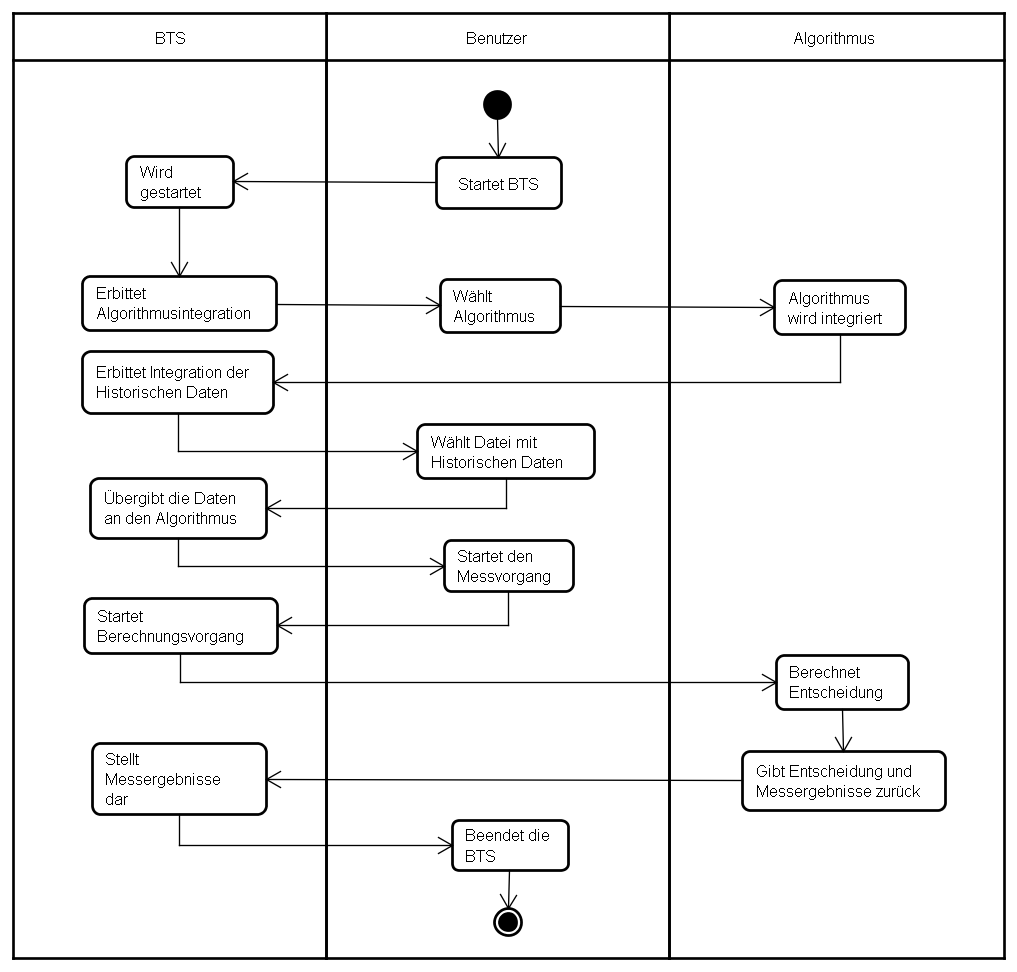
\includegraphics[width=1\textwidth]{graphics/Produktfunktionen/Standardabauf_1.png}
\captionof{figure}{Ein m�glicher Standardablauf von Noctua}}
\end{minipage}

%
% !TeX root = ../Noctua_Pflichtenheft.tex

% Chapter4
\chapter{Produktdaten} \label{chapter:Produktdaten}
/D010/ \textbf{Historische Kursdaten}\\
Historische Kursdaten mehrerer Aktien, sowohl f�r die Algorithmus-Entwicklung als auch f�r
die Backtesting-Software, sollen gespeichert werden.\\
\\
/D020/ \textbf{Algorithmen}\\
Um auch r�ckwirkend auf �ltere oder andere Versionen der Algorithmen zugreifen zu
k�nnen, um beispielsweise Teile davon in neue Versionen zu implementieren oder
auf �ltere Versionen zur�ckzustellen, m�ssen diese inklusive der n�tigen Zusatzinformationen
gespeichert werden.\\
\\
/D030/ \textbf{Algorithmen-Performance-Mapping}\\
Die Ergebnisse der Backtesting-Software sollen f�r jede durchgerechnete Version des Algorithmus
gespeichert werden und sollen auch eindeutig wieder zugeordnet werden k�nnen.
Diese Daten k�nnten in Files oder einer Datenbank gespeichert werden.%
% !TeX root = ../Noctua_Pflichtenheft.tex

% Chapter 6: Produktleistungen

\chapter{Produktleistungen} \label{chapter:produktleistungen}
\section{Leistungen des Algorithmus}

/L10/\\
\emph{Minimale Performance}\\
Die Performance des Algorithmus soll statistisch �ber die letzten 3 Jahre einen h�heren Ertrag erzielen, als der risikofreie Zinssatz. Dies soll am Beispiel von 3 �blichen Aktien oder Aktienindizes nachgewiesen werden.\\

% Geschwindigkeit?

\section{Leistungen der Backtesting-Software}

/L20/\\
\emph{Backtesting Kursdaten}\\
In der \gls{bts} sollen mindestens 3 verschiedene Aktienkurse zur Verf�gung stehen, wobei mindestens einer ein Index sein soll.\\
\\
/L30/\\
\emph{Verwendete Daten}\\
Der Algorithmus darf keine zur Zeit noch nicht vorhandenen Informationen zur Entscheidungsfindung verwenden, da dadurch keine Realsituation simuliert wird und keine Informationen zum Echtzeitbetrieb gewonnen werden.

% Was wir alles im Projekt testen m�ssen: sinnvoll als Leistungen zu definieren?
\section{Projektbezogene Leistungen}

Die folgenden Leistungen m�ssen im Laufe des Projektes erf�llt werden und m�ssen sich, abh�ngig von den Ergebnissen, nicht zwangsweise auf das Produkt auswirken.\\
\\
/L40/\\
\emph{Double MA Crossing}\\
Testen der Performance eines Handelssystems mit 2 \glspl{sma}, sowie 2 \glspl{ema}, die durch Kreuzungen Entscheidungen treffen.\\
\\
/L50/\\
\emph{Triple MA Crossing}\\
Testen eines Handelssystems mit 3 beliebigen \glspl{ma}, die durch definierte Stellung zueinander Entscheidungen treffen.\\
\\
/L60/\\
\emph{Support \& Resistance}\\
Testen der Auswirkungen von der Integration von Support- und Resistance-Mechanismen in das Handelssystem.%


\addcontentsline{toc}{chapter}{Glossary} 
\printglossary[type=\acronymtype]
\glsaddall

\printglossary[type=\acronymtype]
%\printglossary[type=\acronymtype,style=listwithwidth]

%% include appendix
\begin{appendix}
\chapter{Benutzerhandbuch\label{appendix_A}}

%!TEX root=../Benutzerhandbuch.tex
\chapter{Einleitung}
Im Verlauf des Maturaprojekts des 5. Jahrgangs der Abteilung IT am TGM wurde von dem Projektteam Peer Nagy, Gabriel Pawlowsky und Josef Sochovsky unter der Betreuung von Prof. Mag. Hans Brabenetz und Dr. Helmut Vana eine Software geschrieben. Der Sinn und Zweck dieser Software ist das Testen eines Algorithmus �ber eine Menge an gegebenen Daten. Ein solcher Algorithmus ist eine automatisierte Entscheidungslogik, die anhand von historischen Aktiendaten Entscheidungen generieren kann. Eine Entscheidung kann eine Kauf- oder Verkaufsentscheidung. \\
Die Software zeigt Qualit�tsmerkmale des Algorithmus �ber die gegebenen Daten an und simuliert somit einen B�rsenablauf.

%!TEX root=../Benutzerhandbuch.tex
\chapter{Installation}
\section{Start der Installation}
Die Installation wird durch das ausführen der setup.exe gestartet. Danach öffnet sich der Installer.
\begin{figure}[H]
\centering
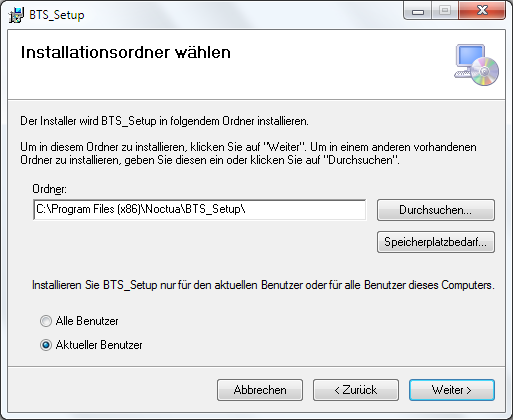
\includegraphics[width=1\textwidth]{images/btsinstall1.png}
\caption{Konfigurieren der Installtion}
\end{figure}
Nach der korrekten Konfiguration des Setups kann die Installtion gestartet werden.
\begin{figure}[H]
\centering
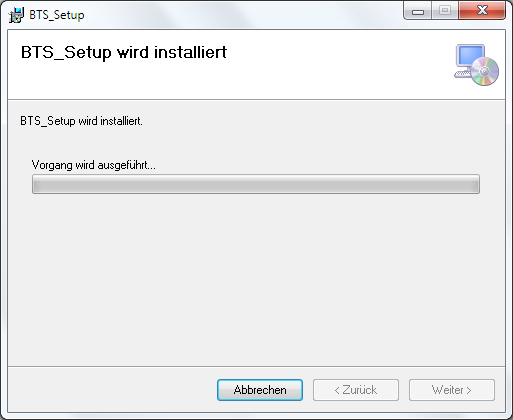
\includegraphics[width=1\textwidth]{images/btsinstall2.png}
\caption{Installationsvorgang}
\end{figure}
Nach diesem Vorgang ist die Backtesting-Software vollständig installiert und ausführbar.
%!TEX root=../Benutzerhandbuch.tex
\section{Programm}
%!TEX root=../../Benutzerhandbuch.tex
\section{Schreiben eines Algorithmus}
Um die Software zu bedienen wird ein in \gls{F-Sharp} geschriebener Algorithmus benötigt. Dieser muss als \gls{DLL}-Datei zur Laufzeit in die Software eingebunden werden. Eine solche Datei wird mittels Microsoft Visual Studio erzeugt werden, damit die Software funktionieren soll. \\
Folgende Eigenschaften muss die Datei erfüllen:
\begin{itemize}
	\item Name der Methode: startCalculation
	\item Übergabeparameter 1: eine Liste aller historischen Daten 
	\item Übergabeparameter 2: eine Liste der Signale für die Entscheidungen (bei Übergabe ist diese Liste leer)
\end{itemize}
Mit dem Rückgabewert der Methode wird nicht gearbeitet, sondern mit der vom Algorithmus verarbeiteten Signalliste.

\begin{lstlisting}[caption=Dateityp des 1. Übergabeparameters]{prices}
System.Collections.Generic.List<System.Tuple
<System.DateTime,decimal,decimal,decimal,decimal>>
\end{lstlisting}
\begin{lstlisting}[caption=Dateityp des 2. Übergabeparameters]{signals}
System.Collections.Generic.List<int>
\end{lstlisting}
Außerdem muss sich der Algorithmus im Namespace  "`Algorithm"' und im Modul "`DecisionCalculator"' befinden.
\subsection{Erzeugen eines Algorithmus-Files}
Öffnen Sie Microsoft Visual Studio und erzeugen sie ein neues Projekt.\\
\begin{figure}[H]
\centering
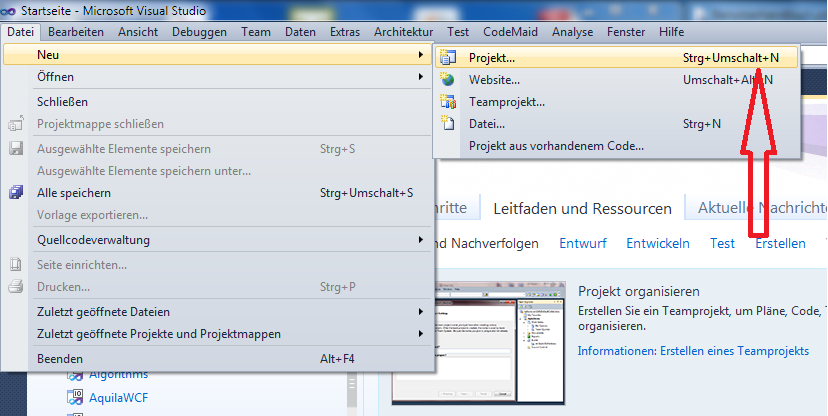
\includegraphics[width=1\textwidth]{images/newProject.png}
\caption{Erzeugen eines neuen Projekts}
\end{figure} 
\newpage
Erstellen Sie es als \gls{F-Sharp}-Bibliothek.
\begin{figure}[H]
\centering
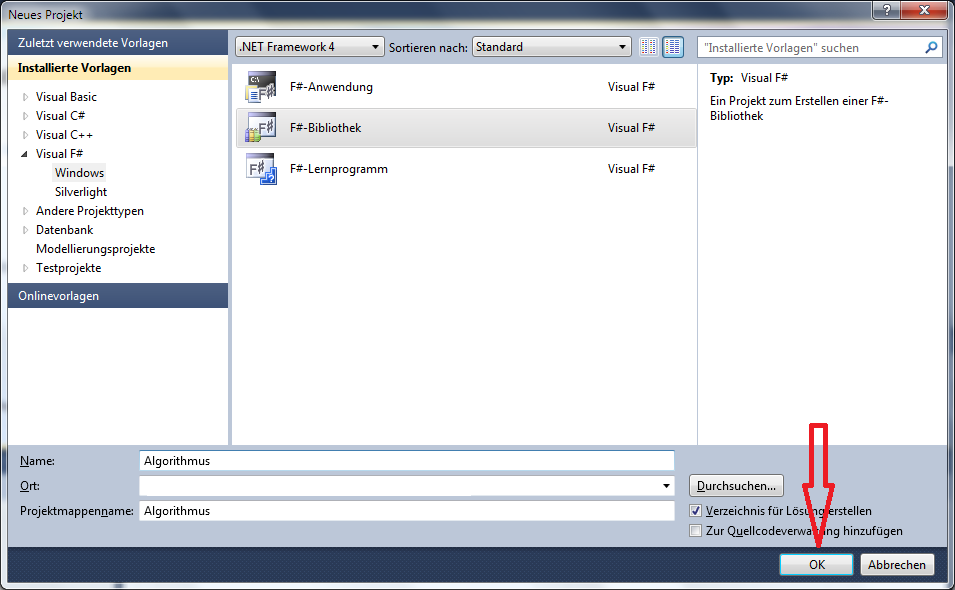
\includegraphics[width=1\textwidth]{images/createProject.png}
\caption{Erstellen Sie es als \gls{F-Sharp}-Bibliothek}
\end{figure}
Halten Sie sich an die, im Kapitel "`Schreiben eines Algorithmus"', genannten Richtlinien und implementieren die Methode startCalculation und kompilieren sie das Projekt.
\begin{figure}[H]
\centering
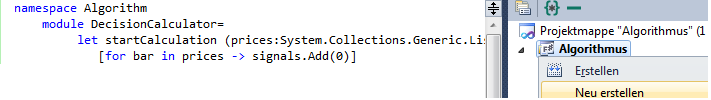
\includegraphics[width=1\textwidth]{images/makeFs.png}
\caption{Kompilieren des Projekts}
\end{figure}
\clearpage
\subsection{Entscheidungen}
Folgende Entscheidungen sind zulässig:
\begin{center}
\begin{tabular}{ |  p{1cm} | p{8cm} |}
\hline 
3 & starkes Kaufssignal \\ \hline
2 &   mittleres Kaufssignal \\ \hline
1 &  schwaches Kaufssignal\\ \hline
0 &  Alle Bestände werden gekauft oder verkauft\\ \hline
-1 &  schwaches Verkaufssignal\\ \hline
-2 &  mittleres Verkaufssignal\\ \hline
-3 &  starkes Verkaufssignal\\ \hline
\end{tabular}
\end{center}

%!TEX root=../../Benutzerhandbuch.tex
\section{Historische Daten}

Um einen Algorithmus mit der \gls{BTS} testen zu k�nnen, m�ssen auch noch historische Aktien-Preisdaten in die Software eingebunden werden, �ber die der Algorithmus getestet wird. Diese k�nnen in Form einer \gls{CSV}-Datei gespeichert und ihr Pfad in der \gls{BTS} angegeben werden. Dabei wurde ein sehr weit verbreitetes Format benutzt, das bspw. auch jegliche Software des renomierten Aktiendatenbereitstellungs-Unternehmens eSignal exportieren kann. Au�erdem werden in dieser Datei die historischen Daten in Form von \glspl{Bar} �ber einen bestimmten Zeitraum (z.B. Daily-\gls{Bar} oder Minute-\gls{Bar}) erwartet und nicht als einzelne Preiswerte. Das Format sieht in etwa so aus:

\begin{lstlisting}[caption=Aufbau der \gls{CSV}-Datei]{csv}
Bar,Date,Time,Open,High,Low,Close
1,01/02/90,00:00,8.8125,9.375, 8.75,9.3125
2,01/03/90,00:00,9.375, 9.50,9.375,9.375
3,01/04/90,00:00,9.375,9.6875,9.3125,9.40625
...
\end{lstlisting}

Zuerst steht also die Nummer des Bars, die allerdings nicht ber�cksichtigt wird. Darauf folgt das Datum in der Form \inline{MM/DD/YY} und die Uhrzeit in der Form \inline{hh:mm}. Zu guter Letzt kommen nun nur noch die Werte Open, High, Low und Close des \glspl{Bar}. Diese Datei kann nahezu unendlich lange gemacht werden, es k�nnen also nahezu unendlich viele Bars nach unten hin erg�nzt werden. Die erste Zeile der Datei wird im Allgemeinen nicht ber�cksichtigt, da sie meist die �berschriften enth�lt. Sollte sich in der ersten Zeile also ein Bar befinden, wird dieser ebenfalls ignoriert.
%!TEX root=../../Benutzerhandbuch.tex
\section{Backtestingsoftware}

Die \gls{BTS} ist nun also die Kernsoftware, mit der die Algorithmen �ber Daten-Files getestet werden k�nnen. Dazu sollten zuerst die allgemeinen Einstellungen get�tigt werden. Diese befinden sich im Settings-Tab unter ''Orders'' und sehen so aus:

\begin{figure}[H]
\centering
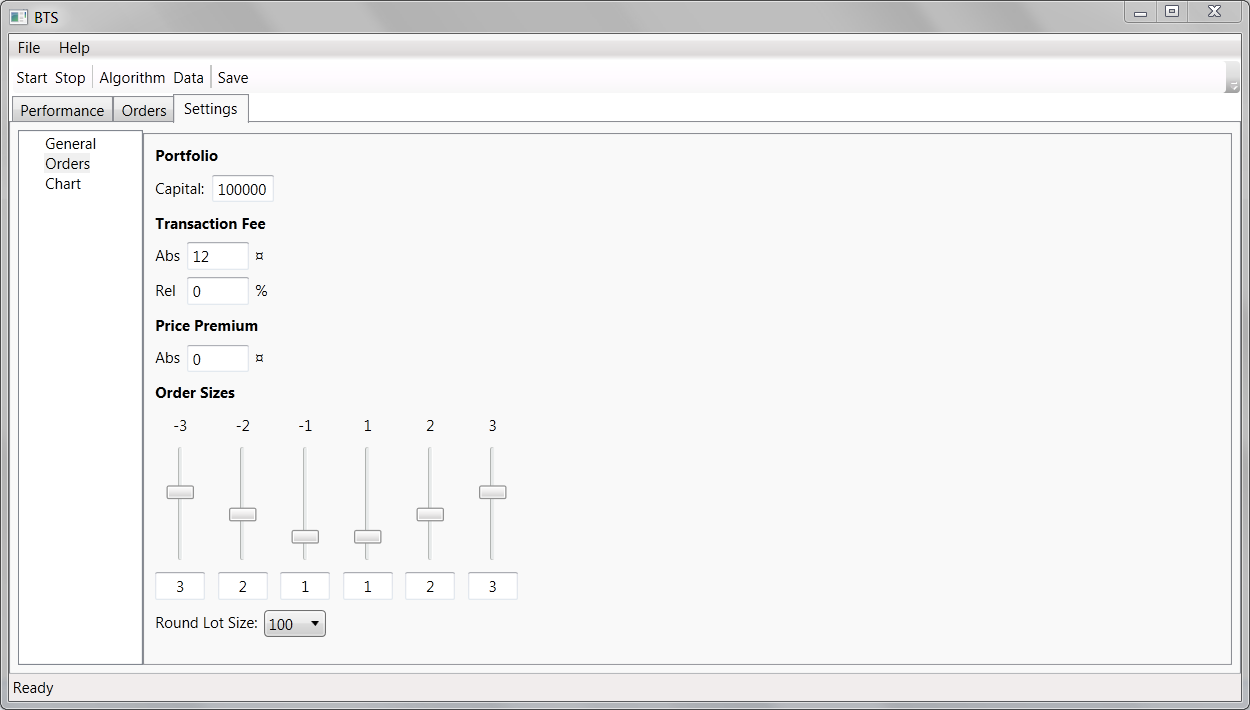
\includegraphics[width=1\textwidth]{images/btsordersettings.png}
\caption{Order-Settings der \gls{BTS}}
\end{figure}

Hier kann zuerst das gew�nschte Kapital eingestellt werden, dessen Handel die \gls{BTS} simulieren soll. Danach k�nnen Transaktionsgeb�hren absolut oder relativ, ein Preisaufschlag f�r K�ufe und die Order-Gr��en eingestellt werden. Die Order-Gr��en geben an, wie viele Round Lots bei einem Signal von -3 bis +3 gekauft/verkauft werden sollen. Ein Round Lot ist hierbei die kleinste �ber einen Online-Broker erwerbbare Menge an Aktien, die ebenfalls variieren und daher eingestellt werden kann.\\ \\

Auf der Seite darunter, der ''Chart''-Seite, k�nnen verschiedene Indikatoren aus der Combobox ausgew�hlt und hinzugef�gt werden, die dann nach der Performancemessung in die Grafik im Orders-Tab eingezeichnet werden. Hier k�nnen au�erdem f�r jeden Indikator die entsprechend notwendigen Parameter und Farben ausgew�hlt werden.

\begin{figure}[H]
\centering
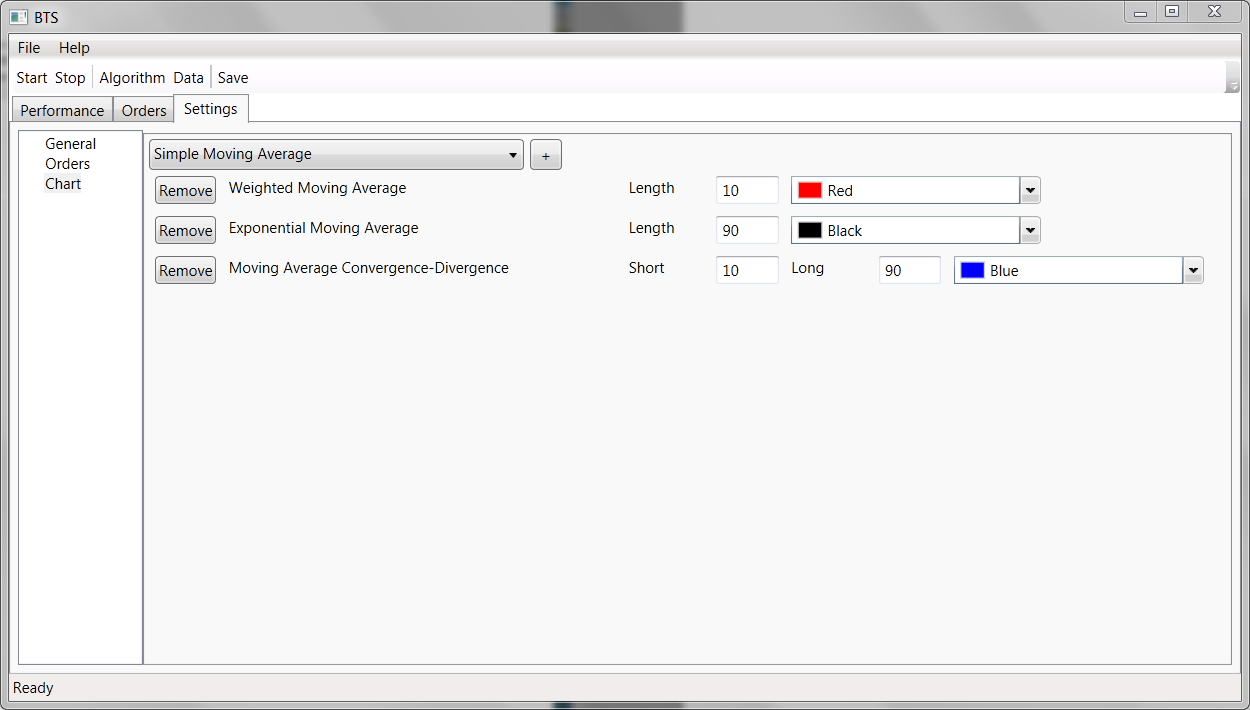
\includegraphics[width=1\textwidth]{images/btschartsettings.png}
\caption{Chart-Settings der \gls{BTS}}
\end{figure}

Weiters k�nnen nun unter der Seite ''General'' die eigentlich wichtigsten Informationen festgelegt werden. Diese sind die Pfade zur Algorithmus- und zur Daten-Datei, die in den vorherigen Punkten erl�utert wurden. Diese Pfade k�nnen �brigens auch durch den ''Algorithm''- und den ''Data''-Button in der Men�leiste hinzugef�gt werden. Darunter kann noch eine Zeitspanne ausgew�hlt werden. Der Algorithmus wird dann nur �ber alle Daten getestet, die im Daten-File im gew�hlten Zeitraum vorkommen.

\begin{figure}[H]
\centering
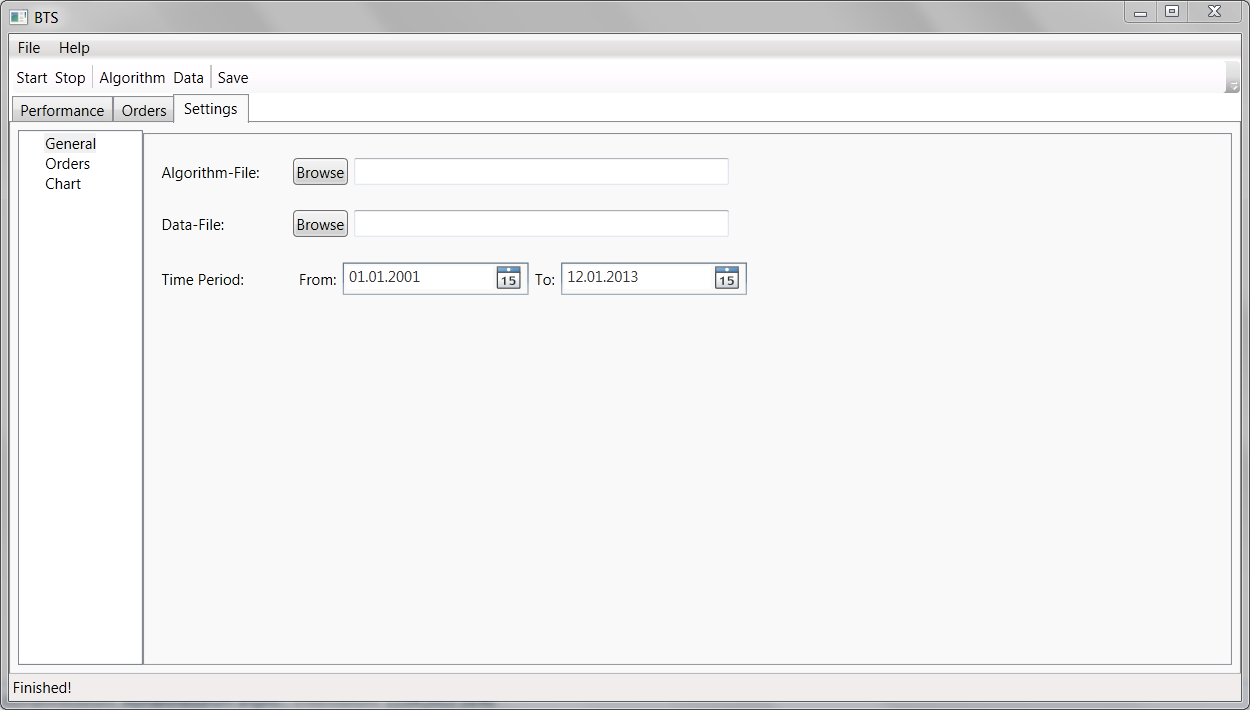
\includegraphics[width=1\textwidth]{images/btsgeneralsettings.png}
\caption{General-Settings der \gls{BTS}}
\end{figure}

Nachdem alle Einstellungen getroffen wurden, kann der Test gestartet werden.

\begin{figure}[H]
\centering
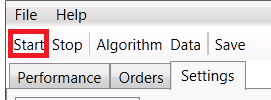
\includegraphics[width=0.6\textwidth]{images/btsstart.png}
\caption{Start-Button der \gls{BTS}}
\end{figure}

Anschlie�end werden auf dem Performance-Tab der \gls{BTS} die allgemeinen Performance-Daten des Algorithmus �ber das spezifizierte Daten-File ausgegeben. N�here Erkl�rungen zu diesen Werten k�nnen durch Halten der Maus �ber einen der Texte als Tooltip angezeigt werden.

\begin{figure}[H]
\centering
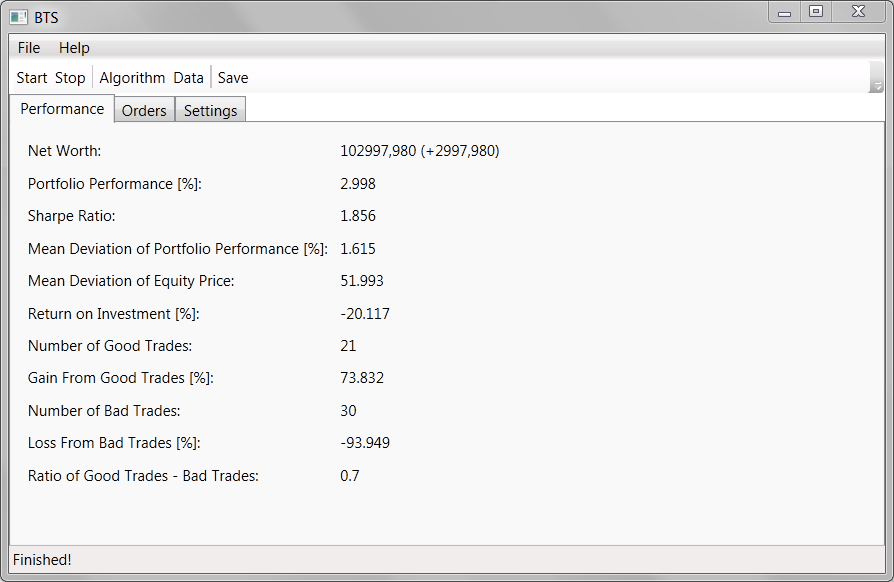
\includegraphics[width=1\textwidth]{images/btsperformance.png}
\caption{Start-Button der \gls{BTS}}
\end{figure}

Die meisten Informationen �ber den Verlauf des Tests k�nnen nun auf dem Orders-Tab gefunden werden. Hier wird zuerst oben ein Chart der Aktien-Preisdaten mit allen gew�hlten Indikatoren angezeigt. Durch Rechtsklick mit der Maus kann im Chart hinausgezoomt und mit der linken Maustaste hineingezoomt werden. Die Pfeile im Chart zeigen an, zu welchen Zeitpunkten der Algorithmus unter reellen Bedingungen �ber den gew�hlten Zeitabschnitt Signale ausgegeben h�tte. Die unterschiedlichen Farben und Farbschattierungen zeigen dabei ein Kauf- (Gr�n) oder ein Verkauf-Signal (Rot) und dessen St�rke an.\\
In der unteren H�lte des Bildschirms wird zu jedem dieser Signale ausgegeben welchen Effekt das jeweilige Signal auf das Kapital h�tte und welcher Gewinn oder Verlust dadurch zum damaligen Preis entstanden w�re. Position bzw. der Transaction Price geben dabei an, wieviele Round Lots durch dieses Signal gekauft worden w�ren und wieviel die Umsetzung des Signals kosten w�rde. Gain/Loss bezieht sich auf die prozentuelle Ver�nderung des Investitionskapitals der expliziten Order und Portfolio Performance auf die prozentuelle bzw. absolute Ver�nderung des gesamten gew�hlten Kapitals. All diese Werte werden auch kumulativ, also aufaddiert, angezeigt. 

\begin{figure}[H]
\centering
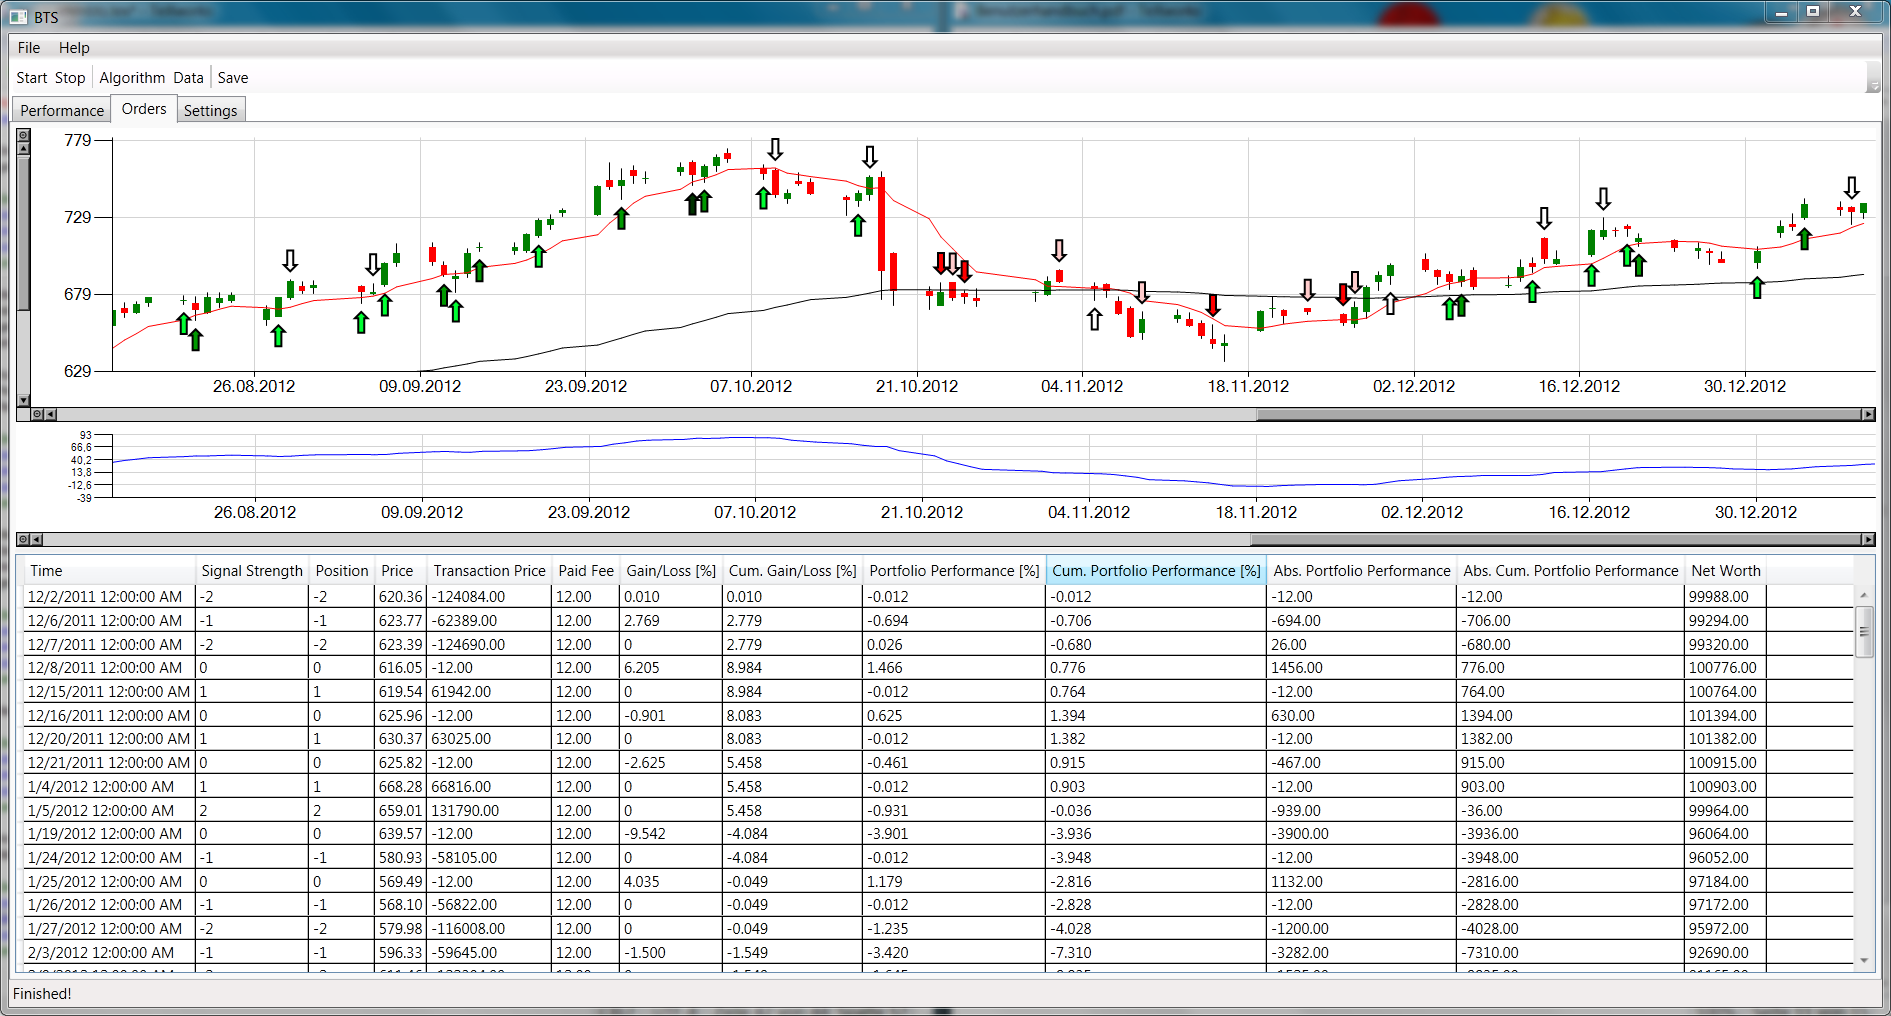
\includegraphics[width=1\textwidth]{images/btsorders.png}
\caption{Start-Button der \gls{BTS}}
\end{figure}

Zu guter Letzt k�nnen unter ''File'' -> ''Export'' die berechneten Performance-Daten lesbar als Text-File (.txt) exportiert werden. Au�erdem kann der aktuelle Zustand der \gls{BTS} inklusive aller Settings und berechneter Daten au�er der Charts (da sonst die Aktiendaten mitgespeichert werden m�ssten) gespeichert und zu einem sp�teren Zeitpunkt erneut geladen werden.
%!TEX root=../Benutzerhandbuch.tex
\chapter{Minimale Systemvoraussetzungen}
Folgende Vorraussetzungen m�ssen vom System erf�llt werden:\\
\textbf{Hardwareanforderungen}
\begin{center}
\begin{tabular}{ | l | c |}\hline 
Prozessor & 1 GHz \\ \hline
RAM & 512 MB \\ \hline
Festplattenspeicher (32 Bit) & 850 MB \\ \hline
Festplattenspeicher (64 Bit) & 2 GB \\ \hline
\end{tabular}
\end{center}
\textbf{Betriebssystemanforderungen} \\
Unterst�tzte Clientbetriebssysteme sind:
\begin{itemize}
\item Windows 8 (32-Bit- und 64-Bit-Editionen)
\item Windows 7 (32-Bit- und 64-Bit-Editionen)
\item Windows Vista (32-Bit- und 64-Bit-Editionen)
\end{itemize}

%\begin{landscape}

\chapter{Zeitaufzeichnungen}

\begin{figure}
	\centering
		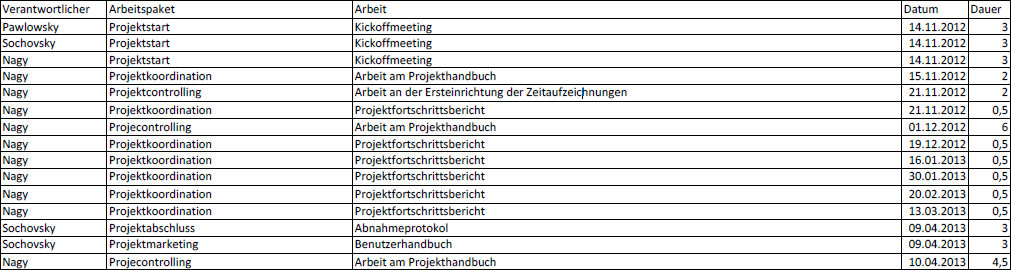
\includegraphics[width=1\textheight, angle=90]{graphics/appendix/projektmanagement.PNG}
	\caption{Projektmanagement}
\end{figure}

\begin{figure}
	\centering
		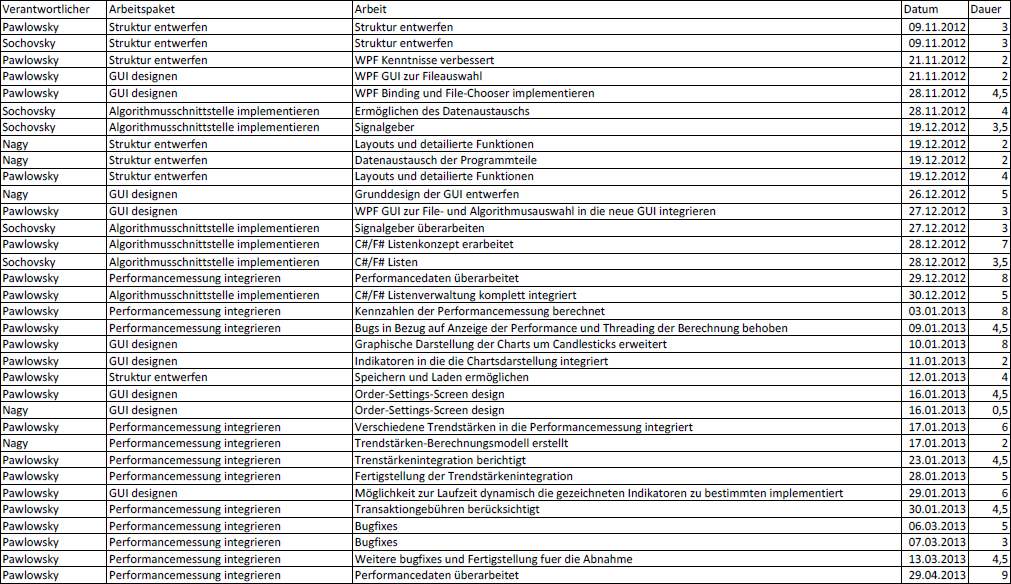
\includegraphics[width=1.0\textheight, angle=90]{graphics/appendix/backtestingsoftware.PNG}
	\caption{Backtesting-Software}
\end{figure}

\begin{figure}
	\centering
		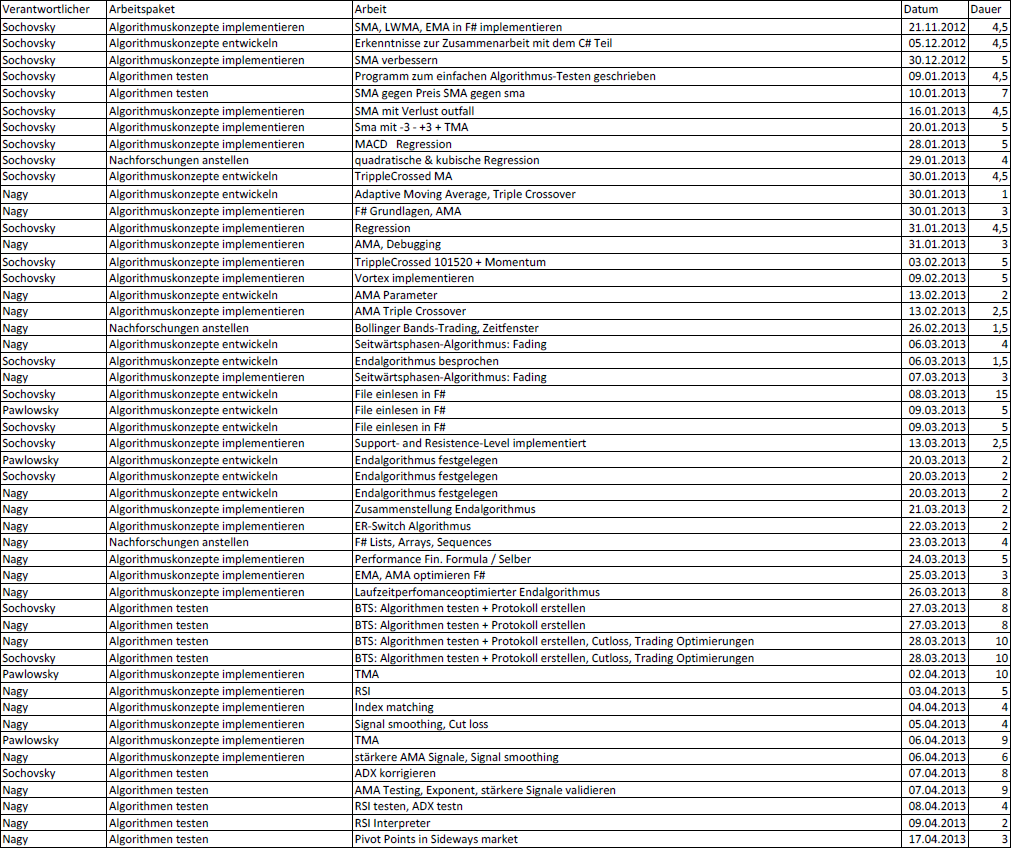
\includegraphics[width=1.0\textheight, angle=90]{graphics/appendix/algorithmus.PNG}
	\caption{Algorithmus}
\end{figure}

\begin{figure}
	\centering
		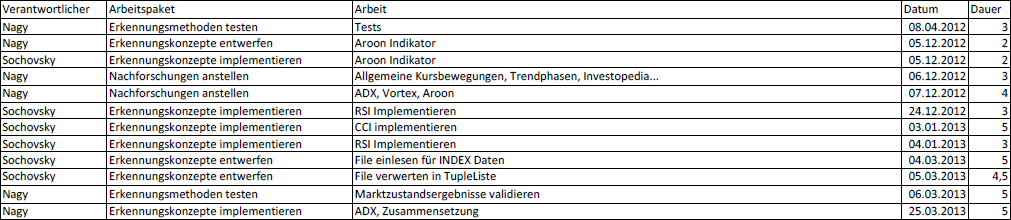
\includegraphics[width=1.0\textheight, angle=90]{graphics/appendix/marktzustandserkennung.PNG}
	\caption{Marktzustandserkennung}
\end{figure}

\begin{figure}
	\centering
		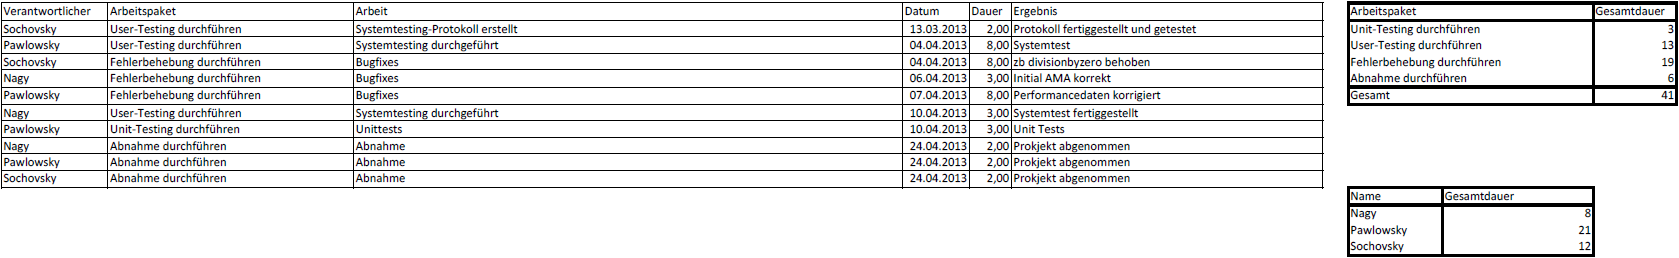
\includegraphics[width=1.0\textheight, angle=90]{graphics/appendix/testingabschluss.PNG}
	\caption{Testing \& Abschluss}
\end{figure}

%\end{landscape}%
\end{appendix}

% Use of the sorted IEEE style, with changes:
% "dashification" was disabled


\cleardoublepage

% IEEE Style
\bibliographystyle{sty/IEEEtranS}

% GATHER
%\input "literatur/bib.bib"
\phantomsection{}
\addcontentsline{toc}{chapter}{\bibname}
\pagestyle{myheadings}\markboth{\bibname}{\bibname}
%\bibliography{bib}

%%% generate index
%\clearpage%
%\markboth{\indexname}{\indexname}%
%\printindex%
%\addcontentsline{toc}{chapter}{\numberline{}\indexname}%

%% include affidavit
\thispagestyle{empty}
\vspace*{2cm}
\begin{center}
{\bf \sf \huge Erkl{\"a}rung}
\end{center}
{\sf \vspace{1cm} Hiermit erkl{\"a}ren wir, dass die vorliegende
Arbeit ohne unzul{\"a}ssige Hilfe Dritter und ohne Benutzung
anderer als der angegebenen Hilfsmittel angefertigt wurde. Die aus
anderen Quellen oder indirekt �bernommenen Daten und Konzepte sind
unter Angabe der Quelle gekennzeichnet.

Die Arbeit wurde bisher weder im In- noch im Ausland in gleicher
oder in {\"a}hnlicher Form in anderen Pr{\"u}fungsverfahren
vorgelegt.
\\[1.5cm]
Wien, im \monthdis
\\[2cm]
Name1
\\[2cm]
Name2
\\[2cm]
Name3
\\[2cm]
Name4
\\[2cm]
}%end sf
%



\end{document}
%%%%%%%%%%%%%%%%%%%%%%%%%%%%%%%%%%%%%%%%%%%%%%%%%%%%%%%%%%%%%%%%%%%%%%%%%%%%%%%%%%%%%%%%%%%%%%%%%%%
%%%%%%%%%%%%%%%%%%%%%%%%%%%%%%%%%%%%%%%%%% End Dokument %%%%%%%%%%%%%%%%%%%%%%%%%%%%%%%%%%%%%%%%%%%
%%%%%%%%%%%%%%%%%%%%%%%%%%%%%%%%%%%%%%%%%%%%%%%%%%%%%%%%%%%%%%%%%%%%%%%%%%%%%%%%%%%%%%%%%%%%%%%%%%%
